% Generated by Sphinx.
\def\sphinxdocclass{report}
\documentclass[letterpaper,10pt,english]{sphinxmanual}
\usepackage[utf8]{inputenc}
\DeclareUnicodeCharacter{00A0}{\nobreakspace}
\usepackage[T1]{fontenc}
\usepackage{babel}
\usepackage{times}
\usepackage[Bjarne]{fncychap}
\usepackage{longtable}
\usepackage{sphinx}
\usepackage{multirow}


\title{Diamond Advanced Planning System Version 8 Documentation}
\date{August 01, 2020}
\release{8}
\author{Jim Schmidt}
\newcommand{\sphinxlogo}{}
\renewcommand{\releasename}{Release}
\makeindex

\makeatletter
\def\PYG@reset{\let\PYG@it=\relax \let\PYG@bf=\relax%
    \let\PYG@ul=\relax \let\PYG@tc=\relax%
    \let\PYG@bc=\relax \let\PYG@ff=\relax}
\def\PYG@tok#1{\csname PYG@tok@#1\endcsname}
\def\PYG@toks#1+{\ifx\relax#1\empty\else%
    \PYG@tok{#1}\expandafter\PYG@toks\fi}
\def\PYG@do#1{\PYG@bc{\PYG@tc{\PYG@ul{%
    \PYG@it{\PYG@bf{\PYG@ff{#1}}}}}}}
\def\PYG#1#2{\PYG@reset\PYG@toks#1+\relax+\PYG@do{#2}}

\def\PYG@tok@gd{\def\PYG@tc##1{\textcolor[rgb]{0.63,0.00,0.00}{##1}}}
\def\PYG@tok@gu{\let\PYG@bf=\textbf\def\PYG@tc##1{\textcolor[rgb]{0.50,0.00,0.50}{##1}}}
\def\PYG@tok@gt{\def\PYG@tc##1{\textcolor[rgb]{0.00,0.25,0.82}{##1}}}
\def\PYG@tok@gs{\let\PYG@bf=\textbf}
\def\PYG@tok@gr{\def\PYG@tc##1{\textcolor[rgb]{1.00,0.00,0.00}{##1}}}
\def\PYG@tok@cm{\let\PYG@it=\textit\def\PYG@tc##1{\textcolor[rgb]{0.25,0.50,0.56}{##1}}}
\def\PYG@tok@vg{\def\PYG@tc##1{\textcolor[rgb]{0.73,0.38,0.84}{##1}}}
\def\PYG@tok@m{\def\PYG@tc##1{\textcolor[rgb]{0.13,0.50,0.31}{##1}}}
\def\PYG@tok@mh{\def\PYG@tc##1{\textcolor[rgb]{0.13,0.50,0.31}{##1}}}
\def\PYG@tok@cs{\def\PYG@tc##1{\textcolor[rgb]{0.25,0.50,0.56}{##1}}\def\PYG@bc##1{\colorbox[rgb]{1.00,0.94,0.94}{##1}}}
\def\PYG@tok@ge{\let\PYG@it=\textit}
\def\PYG@tok@vc{\def\PYG@tc##1{\textcolor[rgb]{0.73,0.38,0.84}{##1}}}
\def\PYG@tok@il{\def\PYG@tc##1{\textcolor[rgb]{0.13,0.50,0.31}{##1}}}
\def\PYG@tok@go{\def\PYG@tc##1{\textcolor[rgb]{0.19,0.19,0.19}{##1}}}
\def\PYG@tok@cp{\def\PYG@tc##1{\textcolor[rgb]{0.00,0.44,0.13}{##1}}}
\def\PYG@tok@gi{\def\PYG@tc##1{\textcolor[rgb]{0.00,0.63,0.00}{##1}}}
\def\PYG@tok@gh{\let\PYG@bf=\textbf\def\PYG@tc##1{\textcolor[rgb]{0.00,0.00,0.50}{##1}}}
\def\PYG@tok@ni{\let\PYG@bf=\textbf\def\PYG@tc##1{\textcolor[rgb]{0.84,0.33,0.22}{##1}}}
\def\PYG@tok@nl{\let\PYG@bf=\textbf\def\PYG@tc##1{\textcolor[rgb]{0.00,0.13,0.44}{##1}}}
\def\PYG@tok@nn{\let\PYG@bf=\textbf\def\PYG@tc##1{\textcolor[rgb]{0.05,0.52,0.71}{##1}}}
\def\PYG@tok@no{\def\PYG@tc##1{\textcolor[rgb]{0.38,0.68,0.84}{##1}}}
\def\PYG@tok@na{\def\PYG@tc##1{\textcolor[rgb]{0.25,0.44,0.63}{##1}}}
\def\PYG@tok@nb{\def\PYG@tc##1{\textcolor[rgb]{0.00,0.44,0.13}{##1}}}
\def\PYG@tok@nc{\let\PYG@bf=\textbf\def\PYG@tc##1{\textcolor[rgb]{0.05,0.52,0.71}{##1}}}
\def\PYG@tok@nd{\let\PYG@bf=\textbf\def\PYG@tc##1{\textcolor[rgb]{0.33,0.33,0.33}{##1}}}
\def\PYG@tok@ne{\def\PYG@tc##1{\textcolor[rgb]{0.00,0.44,0.13}{##1}}}
\def\PYG@tok@nf{\def\PYG@tc##1{\textcolor[rgb]{0.02,0.16,0.49}{##1}}}
\def\PYG@tok@si{\let\PYG@it=\textit\def\PYG@tc##1{\textcolor[rgb]{0.44,0.63,0.82}{##1}}}
\def\PYG@tok@s2{\def\PYG@tc##1{\textcolor[rgb]{0.25,0.44,0.63}{##1}}}
\def\PYG@tok@vi{\def\PYG@tc##1{\textcolor[rgb]{0.73,0.38,0.84}{##1}}}
\def\PYG@tok@nt{\let\PYG@bf=\textbf\def\PYG@tc##1{\textcolor[rgb]{0.02,0.16,0.45}{##1}}}
\def\PYG@tok@nv{\def\PYG@tc##1{\textcolor[rgb]{0.73,0.38,0.84}{##1}}}
\def\PYG@tok@s1{\def\PYG@tc##1{\textcolor[rgb]{0.25,0.44,0.63}{##1}}}
\def\PYG@tok@gp{\let\PYG@bf=\textbf\def\PYG@tc##1{\textcolor[rgb]{0.78,0.36,0.04}{##1}}}
\def\PYG@tok@sh{\def\PYG@tc##1{\textcolor[rgb]{0.25,0.44,0.63}{##1}}}
\def\PYG@tok@ow{\let\PYG@bf=\textbf\def\PYG@tc##1{\textcolor[rgb]{0.00,0.44,0.13}{##1}}}
\def\PYG@tok@sx{\def\PYG@tc##1{\textcolor[rgb]{0.78,0.36,0.04}{##1}}}
\def\PYG@tok@bp{\def\PYG@tc##1{\textcolor[rgb]{0.00,0.44,0.13}{##1}}}
\def\PYG@tok@c1{\let\PYG@it=\textit\def\PYG@tc##1{\textcolor[rgb]{0.25,0.50,0.56}{##1}}}
\def\PYG@tok@kc{\let\PYG@bf=\textbf\def\PYG@tc##1{\textcolor[rgb]{0.00,0.44,0.13}{##1}}}
\def\PYG@tok@c{\let\PYG@it=\textit\def\PYG@tc##1{\textcolor[rgb]{0.25,0.50,0.56}{##1}}}
\def\PYG@tok@mf{\def\PYG@tc##1{\textcolor[rgb]{0.13,0.50,0.31}{##1}}}
\def\PYG@tok@err{\def\PYG@bc##1{\fcolorbox[rgb]{1.00,0.00,0.00}{1,1,1}{##1}}}
\def\PYG@tok@kd{\let\PYG@bf=\textbf\def\PYG@tc##1{\textcolor[rgb]{0.00,0.44,0.13}{##1}}}
\def\PYG@tok@ss{\def\PYG@tc##1{\textcolor[rgb]{0.32,0.47,0.09}{##1}}}
\def\PYG@tok@sr{\def\PYG@tc##1{\textcolor[rgb]{0.14,0.33,0.53}{##1}}}
\def\PYG@tok@mo{\def\PYG@tc##1{\textcolor[rgb]{0.13,0.50,0.31}{##1}}}
\def\PYG@tok@mi{\def\PYG@tc##1{\textcolor[rgb]{0.13,0.50,0.31}{##1}}}
\def\PYG@tok@kn{\let\PYG@bf=\textbf\def\PYG@tc##1{\textcolor[rgb]{0.00,0.44,0.13}{##1}}}
\def\PYG@tok@o{\def\PYG@tc##1{\textcolor[rgb]{0.40,0.40,0.40}{##1}}}
\def\PYG@tok@kr{\let\PYG@bf=\textbf\def\PYG@tc##1{\textcolor[rgb]{0.00,0.44,0.13}{##1}}}
\def\PYG@tok@s{\def\PYG@tc##1{\textcolor[rgb]{0.25,0.44,0.63}{##1}}}
\def\PYG@tok@kp{\def\PYG@tc##1{\textcolor[rgb]{0.00,0.44,0.13}{##1}}}
\def\PYG@tok@w{\def\PYG@tc##1{\textcolor[rgb]{0.73,0.73,0.73}{##1}}}
\def\PYG@tok@kt{\def\PYG@tc##1{\textcolor[rgb]{0.56,0.13,0.00}{##1}}}
\def\PYG@tok@sc{\def\PYG@tc##1{\textcolor[rgb]{0.25,0.44,0.63}{##1}}}
\def\PYG@tok@sb{\def\PYG@tc##1{\textcolor[rgb]{0.25,0.44,0.63}{##1}}}
\def\PYG@tok@k{\let\PYG@bf=\textbf\def\PYG@tc##1{\textcolor[rgb]{0.00,0.44,0.13}{##1}}}
\def\PYG@tok@se{\let\PYG@bf=\textbf\def\PYG@tc##1{\textcolor[rgb]{0.25,0.44,0.63}{##1}}}
\def\PYG@tok@sd{\let\PYG@it=\textit\def\PYG@tc##1{\textcolor[rgb]{0.25,0.44,0.63}{##1}}}

\def\PYGZbs{\char`\\}
\def\PYGZus{\char`\_}
\def\PYGZob{\char`\{}
\def\PYGZcb{\char`\}}
\def\PYGZca{\char`\^}
\def\PYGZsh{\char`\#}
\def\PYGZpc{\char`\%}
\def\PYGZdl{\char`\$}
\def\PYGZti{\char`\~}
% for compatibility with earlier versions
\def\PYGZat{@}
\def\PYGZlb{[}
\def\PYGZrb{]}
\makeatother

\begin{document}

\maketitle
\tableofcontents
\phantomsection\label{index::doc}



\chapter{Objectives}
\label{FutureState:objectives}\label{FutureState::doc}\label{FutureState:future-state}\begin{enumerate}
\item {} 
Maximum buyer productivity

\item {} 
Eliminate unnecessary purchases

\item {} 
Develop a standardized methodology for buyers that is deterministic,
with the same input two buyers should come to the same conclusions.

\item {} 
Buyers should be able to test the results of a simulation by, for
example adding a secondary manufacturer CofC to a lot and replan the
part and get the answer back within a second with a new single
screen.

\item {} 
All scenarios should be stored with the results.

\item {} 
Upon acceptance of a scenario the simulation changes should be
reported so that the source systems can be update.

\item {} 
Status of simulation changes \# Requested \# Not possible - stops
further recommendations to take this action \# Active - Once a
download from the source system reflects this change

\item {} 
A report of requested modification not yet completed on source
systems

\end{enumerate}


\chapter{Purchasing Operational Efficiency}
\label{FutureState:purchasing-operational-efficiency}

\section{Purchasing Review Board}
\label{FutureState:purchasing-review-board}
Requisitions may be reviewed by the purchasing review board
\begin{itemize}
\item {} 
Approval

\item {} 
Disapproval

\item {} 
Record disapproval reason for requisitions Purchasing review board

\end{itemize}

can select (or create and select) a reason such as:
\begin{itemize}
\item {} \begin{description}
\item[{Review equivalent parts}] \leavevmode\begin{itemize}
\item {} 
Is onhand under another part

\item {} 
insufficient quotations (other vendors may have lower costs)

\end{itemize}

\end{description}

\end{itemize}


\section{Speed up quotations}
\label{FutureState:speed-up-quotations}\begin{itemize}
\item {} 
Automatically email vendors request for quotations

\item {} 
Automated quote response have the vendors provide a CSV, JSON or XML
file with the quote to be automatically uploaded to the system.

\end{itemize}

For example a vendor could create a spreadsheet with the following
columns
\begin{itemize}
\item {} 
item\_cd

\item {} 
quantity

\item {} 
manufacturer

\item {} 
price

\item {} 
available date

\end{itemize}

by emailing to \href{mailto:quotes@yourco.com}{quotes@yourco.com} these quotes can be automatically
loaded into the system without changes to the legacy system,


\section{Buyer information}
\label{FutureState:buyer-information}
The buyer should have single screen that shows:
\begin{enumerate}
\item {} 
Supplies

\item {} 
On hand

\item {} 
Open Purchase Orders

\item {} 
Open Work Orders

\item {} 
Demand

\item {} 
Forecasted
\begin{enumerate}
\item {} 
Raw

\item {} 
Consumed

\item {} 
Unconsumed

\end{enumerate}

\item {} 
Safety Stock

\item {} 
Reserved Inventory

\item {} 
Quarantined

\item {} 
Restricted access (JIT programs, Committed Service Level Agreement
Plans)

\item {} 
All part numbers in the planning group

\item {} 
Every part and all equivalents, transitively, that is the equivalents
to those equivalents until exhausted.

\item {} 
Customer specific substitutions

\item {} 
Approved manufacturer matrix Customers down the left, manufacturers
across the top

\item {} 
Requisitions

\item {} 
Supplier on-time historical metrics

\item {} 
Supply ineligibility drill-down

\item {} 
Vendor Quotes

\item {} 
Time phased inventory position, Pipeline (Global, by Facility, by
planner)

\item {} 
On hand inventory in aggregate with the ability to open details with
a single click

\item {} 
Sales history for the last three years in multiple dimensions

\item {} 
Time Dimensions include annual, quarterly and monthly

\item {} 
Ability to see by customer

\item {} 
Existing purchase orders

\item {} 
Existing facility transfers in process

\item {} 
Detailed reason why supplies are not eligible for a demand that is
allocated late or short

\item {} 
A matrix of approved manufactures and customers

\item {} 
See the part and all transitive equivalent parts

\item {} 
Late or short demands

\end{enumerate}

In Diamond this is all done locally in the web browser with no network
requests so it is virtually instantaneous.


\section{Recommendations}
\label{FutureState:recommendations}\begin{enumerate}
\item {} 
Purchase orders that can be cancelled

\item {} 
Get a manufacturer Certificate of Compliance for existing inventory
to satisfy a requisition with existing inventory

\item {} 
Supply prioritization Use buyback inventory before using our
inventory for appropriate customers

\item {} 
Allocation based pricing

\item {} 
Items with a shelf life have oldest allocated first

\item {} 
Less valuable items are allocated first

\item {} 
Based on Certifications (dual certified parts have more value)

\item {} 
Facility Transfer

\item {} 
Supply Pool Transfer

\item {} 
Expedite or de-expedite a purchase order

\end{enumerate}


\section{Alerts}
\label{FutureState:alerts}\begin{itemize}
\item {} 
Obsolete Inventory

\item {} 
Expiring Inventory

\item {} 
Purchase Exceeding x\% of previous maximum unit price

\item {} 
Purchase Exceeding x\% of previous minimum unit price

\item {} 
Purchase of specified dollars not yet approved

\end{itemize}


\chapter{Extensibility}
\label{FutureState:extensibility}
Any component must be easily plugged in with an alternative
implementation that is compliant with the corresponding interface,
\begin{itemize}
\item {} 
Demand Priority

\item {} 
Eligibility Requirements

\item {} 
Supply Prioritization
\begin{itemize}
\item {} 
Lot value determination

\end{itemize}

\item {} 
Recommendation Handlers for propagating accepted recommendations to
source system

\end{itemize}


\chapter{Implementation}
\label{FutureState:implementation}\begin{itemize}
\item {} 
Extract necessary data from legacy systems

\item {} 
Load into Advanced Planning

\item {} 
Augment with necessary but unavailable information

\item {} 
Run a full plan

\item {} 
Review recommendations
\begin{itemize}
\item {} 
Accept recommendation (must define Action Handlers) Reject
recommendation (select reason to be persisted across full reloads)

\end{itemize}

\end{itemize}


\section{Questions}
\label{FutureState:questions}\begin{enumerate}
\item {} 
Inventory Restriction

\item {} 
How do you restrict availability of inventory for special purposes
such as
\begin{itemize}
\item {} 
JIT contracts

\item {} 
Committed Service Level Agreements

\item {} 
Kitting and Assembly

\end{itemize}

\item {} 
Do you have automated approved manufacturer eligibility?

\item {} 
Do you have prioritization for lots with expiry dates?

\item {} 
How do you calculate the residual cost of goods for broker buys for
the

\item {} 
Are you exclusively FIFO or do you consider lots that have lower cost
that satisfies the demand (taking into consideration multiple
certifications, incremental cost of Quality Assurance testing and
destructive tests?), etc.? Quantity that exceeds the customer demand?

\item {} 
Quality Assurance Do you have a quality assurance program that
supports skip lot testing and pre-approved lots ( lots that have
already passed the QA requirements for a customer should receive
higher priority for that customer and lower priority for others)

\item {} 
What supply eligibility rules do you have?

\item {} 
How do you pin an allocation to a demand ?

\item {} 
Does your system recommend when alternate availability is preferable
to a pinned allocation?

\end{enumerate}


\section{Simple Example}
\label{FutureState:simple-example}
During one of my calls with Peter he told me that he was reviewing
purchase orders a simple line such as ``Buyers don't buy the correct
quantities to get a good price'' was extended to:


\subsection{Compute Optimal Purchase Quantity}
\label{FutureState:compute-optimal-purchase-quantity}
Compute a projected per unit cost by solving the equation

unit\_cost = (setup\_cost / qty) + incremental cost

For two different known qty and prices (vendor quotes) using linear
algebra


\subsection{Graph this relationsihip}
\label{FutureState:graph-this-relationsihip}
Find the ``price knee'' the first derivative of the function, the slope of
the tangent starts to level off (it asymptotically approaches 0, meaning
the limit is the unit cost doesn't decrease at all. Depending on setup
cost, incremental cost and annual consumption a three year supply may be
ten percent more than a one year supply, it may also be three times the
acquisition cost and additional carrying costs must be considered.

Vendor quotes should include this range of quantities, purchasing
quantities should be in this range, buys can be made and even scheduled
so that lower per unit costs can be realized.


\section{Purchasing Procedures}
\label{FutureState:purchasing-procedures}
When a part needs to be replenished
\begin{enumerate}
\item {} 
Vendor quotes for the price range should be required.

\item {} 
Purchase amounts over a defined limit should be reviewed and
approved.

\item {} 
Requisitions should be created in the new purchase decision
application and once approved, be created as purchase orders in the
execution system (Dymax and SAP).

\item {} 
Checks for any constraints including approved manufacturers should be
simulated

\item {} 
Existing inventory carried under equivalent part numbers should be
considered.

\end{enumerate}

The opportunities for process improvement are best addressed by
evaluating your current processes and the issues your experts realize
and developing a system to address those issues.


\section{Constraints}
\label{FutureState:constraints}
Your new process should:
\begin{enumerate}
\item {} 
Be external to SAP and Dymax, requiring no modifications to either
system. This eliminates risk and complexity.

\item {} 
Should include data from both operations for inventory, purchases and
demands

\item {} 
Incorporate new procedures and policies to reflect best practices

\item {} 
Reduce the effort of sales staff and purchasing staff to perform
their functions

\item {} 
Define metrics to evaluate performance and progress

\item {} 
Have an alert system of reports of issues that need to be addressed.

\item {} 
Require no hardware or other infrastructure or the installation of
any software on any Align computer.

\end{enumerate}


\chapter{Questions}
\label{FutureState:id1}
What is the current cost of
\begin{enumerate}
\item {} 
Not buying the correct quantities

\item {} 
Not taking into consideration multiple certifications

\item {} 
Buying inventory in one operation that is excess inventory in the
other operation

\item {} 
Time wasted gathering information to create a purchase order

\end{enumerate}


\chapter{Conclusion}
\label{FutureState:conclusion}
Align has the expertise in house to participate in the design of a
business process and software to optimize the purchasing and sales
operations, there is no need to wait for an IT person who has much less
experience than your director of purchasing and other operations
personnel.

A one hour phone call every two weeks is not going to ever get you a
design.

I have no doubt that several times every day a sub-optimal purchase
results in a expense greater than the cost of developing a design.

A design is best done by whiteboard meetings, starting with a blank
whiteboard. Even with 25 years experience in Aerospace, it would be
presumption, and flat out wrong for me to give a Powerpoint
presentation and say ``This is the universal answer to all problems, it
will fit your situation''; this is the approach of someone hawking
software.
\begin{itemize}
\item {} 
Automatically email vendors request for quotations

\item {} 
Automated quote response have the vendors provide a CSV, JSON or XML
file with the quote to be

\item {} 
automatically uploaded to the system.

\end{itemize}

For example a vendor could create a spreadsheet with the following
columns
\begin{itemize}
\item {} 
item\_cd

\item {} 
quantity

\item {} 
manufacturer

\item {} 
price

\item {} 
available date

\end{itemize}

by emailing to \href{mailto:quotes@yourco.com}{quotes@yourco.com} these quotes can be automatically
loaded into the system without changes to the legacy system,

The buyer should have single screen that shows:
\begin{enumerate}
\item {} 
Supplies

\item {} 
On hand

\item {} 
Open Purchase Orders

\item {} 
Open Work Orders

\item {} 
Demand

\item {} 
Forecasted
\begin{enumerate}
\item {} 
Raw

\item {} 
Consumed

\item {} 
Unconsumed

\end{enumerate}

\item {} 
Safety Stock

\item {} 
Work Orders

\item {} 
Reserved Inventory

\item {} 
Quarantined

\item {} 
Restricted access (JIT programs, Committed Service Level Agreement
Plans)

\item {} 
All part numbers in the planning group

\item {} 
Every part and all equivalents, transitively, that is the equivalents
to those equivalents until exhausted.

\item {} 
Customer specific substitutions

\item {} 
Approved manufacturer matrix Customers down the left, manufacturers
across the top

\item {} 
Requisitions

\item {} 
Supplier on-time historical metrics

\item {} 
Supply ineligibility drill-down

\item {} 
Vendor Quotes

\item {} 
Time phased inventory position, Pipeline (Global, by Facility, by
planner)

\item {} 
On hand inventory in aggregate with the ability to open details with
a single click

\item {} 
Sales history for the last three years in multiple dimensions

\item {} 
Time Dimensions include annual, quarterly and monthly

\item {} 
Ability to see by customer

\item {} 
Existing purchase orders

\item {} 
Existing facility transfers in process

\item {} 
Detailed reason why supplies are not eligible for a demand that is
allocated late or short

\item {} 
A matrix of approved manufactures and customers

\item {} 
See the part and all transitive equivalent parts

\item {} 
Late or short demands

\end{enumerate}

In Diamond this is all done locally in the web browser with no network
requests so it is virtually instantaneous.


\chapter{Modifications}
\label{FutureState:modifications}\begin{itemize}
\item {} 
All code is in Java supported by Spring with Hibernate for Object
Relation Management, these are widely adoped open source solutions

\item {} 
Presentation uses the Model, View Controller approach and the model
may be exposed as a JavaBean or XML if one prefers to use XSL.

\item {} 
Diamond dependencies are all vastly popular open source but it
extremely unlikely anyone will have any need to modify anyy of the
open source code

\item {} 
I have trained non-programmers to modify Diamond in less than a
month.

\end{itemize}


\section{Questions}
\label{FutureState:id2}\begin{enumerate}
\item {} 
Inventory Restriction

\item {} 
How do you restrict availability of inventory for special purposes
such as
\begin{itemize}
\item {} 
JIT contracts

\item {} 
Committed Service Level Agreements

\item {} 
Kitting and Assembly

\end{itemize}

\item {} 
Do you have automated approved manufacturer eligibility?

\item {} 
Do you have prioritization for lots with expiry dates?

\item {} 
How do you calculate the residual cost of goods for broker buys for
the

\item {} 
Are you exclusively FIFO or do you consider lots that have lower cost
that satisfies the demand (taking into consideration multiple
certifications, incremental cost of Quality Assurance testing and
destructive tests?), etc.? quantity that exceeds the customer demand?

\item {} 
Quality Assurance Do you have a quality assurance program that
supports skip lot testing and pre-approved lots ( lots that have
already passed the QA requirements for a customer should receive
higher priority for that customer and lower priority for others)

\item {} 
What supply eligibility rules do you have?

\item {} 
How do you pin an allocation to a demand ?

\item {} 
Does your system recommend when alternate availability is preferable
to a pinned allocation?

\end{enumerate}


\chapter{Business Process Iprovement}
\label{Introduction/Business-process-improvement::doc}\label{Introduction/Business-process-improvement:business-process-iprovement}
Overhaul all client Business Processes associated with Inventory Planning and the operations necessary to effect that overhaul


\section{Business Process Improvement Description}
\label{Introduction/Business-process-improvement:business-process-improvement-description}
Managed by Thomas Moreno, who wiil working with each department
This describes Business Process Improvement at client

Objectives and Benefits:
\begin{itemize}
\item {} 
Define standardized procedures and tools to

\item {} 
Improve employee productivity (facilitate decision makers and reduce clerical work)

\item {} 
Produce better decisions

\item {} 
Improve cash utilization

\item {} 
Optimize inventory

\item {} 
Produce more consistent results

\item {} 
Grow sales

\item {} 
Document procedures

\item {} 
Audit trails

\item {} 
Share inventory information across holding company units.  Currently US and European operations duplicate work and inventory.

\item {} 
Reduce inventory by using inventory maintained as equivalent parts.

\item {} 
Allow these users to use the new system for better and more efficient decision making while offloading legacy system specific clerical work.

\item {} 
Determinism, with the same input, make similar decisions

\end{itemize}

This initiative will benefit:
\begin{itemize}
\item {} 
Inventory Planners

\item {} 
Buyers

\item {} 
Sellers

\item {} 
Customers

\item {} 
Finance

\end{itemize}


\section{Approach}
\label{Introduction/Business-process-improvement:approach}
Provide a software tool that
\begin{quote}
\begin{itemize}
\item {} 
Design to work as we desired to work

\item {} 
Exception and priority based

\item {} 
User interfackkkkke customized to each area of responsibility

\item {} 
Simplify work

\item {} 
Improve quality with team review

\item {} 
Provide better decision support information

\item {} 
Change procedures to reduce tedious work overheadl

\item {} 
Allow for simplification

\item {} 
Allow the system to work in accordance with policy with maximum efficiency for users

\item {} 
improve inter-company  cooperation

\item {} 
Support proactive activity Additional System Functionality

\end{itemize}
\begin{itemize}
\item {} 
Controls

\item {} 
iiiiiiiiiiiiAs policies are developed the new system will enforce these policies with actions flagged for review to be approved or additional research as necessary.i * Describe current and Future State

\end{itemize}
\end{quote}
\begin{itemize}
\item {} \begin{itemize}
\item {} 
List benefits of future state

\end{itemize}

\end{itemize}


\section{Create tass for future state with}
\label{Introduction/Business-process-improvement:create-tass-for-future-state-with}\begin{quote}

{\color{red}\bfseries{}*}i Describe what kwill be done in the future
* Functional description
* Prioritize tasks

{\color{red}\bfseries{}*}risk / No changes to existing systems
\end{quote}


\section{Document References}
\label{Introduction/Business-process-improvement:document-references}
\href{https://en.wikipedia.org/wiki/Business\_process\_re-engineering}{https://en.wikipedia.org/wiki/Business\_process\_re-engineering}


\chapter{Business Process Improvement : Diamond History}
\label{Introduction/Diamond-History2::doc}\label{Introduction/Diamond-History2:business-process-improvement-diamond-history}\begin{enumerate}
\item {} 
Business Process Improvement

\item {} 
Project Description

\end{enumerate}


\section{Business Process Improvement : Diamond History}
\label{Introduction/Diamond-History2:id1}
Created by James Schmidt, last modified on Dec 21, 2019


\subsection{History}
\label{Introduction/Diamond-History2:history}
The User Interface has been rewritten many times since 1995

Oracle Forms 3

Oracle Forms 4.5

Java Servlets

Java JSP

Oracle Apex

Now being written in Angular 8


\subsubsection{Layout}
\label{Introduction/Diamond-History2:layout}

\subsection{Login}
\label{Introduction/Diamond-History2:login}

\subsection{Action Reports}
\label{Introduction/Diamond-History2:action-reports}

\subsection{Information Reports}
\label{Introduction/Diamond-History2:information-reports}

\subsection{Query}
\label{Introduction/Diamond-History2:query}

\subsection{Item / Plan Group Listing}
\label{Introduction/Diamond-History2:item-plan-group-listing}
Document generated by Confluence on Dec 22, 2019 07:29

\href{http://www.atlassian.com/}{Atlassian}


\chapter{Business Process Improvement : Diamond History}
\label{Introduction/Diamond-History::doc}\label{Introduction/Diamond-History:business-process-improvement-diamond-history}\begin{enumerate}
\item {} 
Business Process Improvement

\item {} 
Project Description

\end{enumerate}


\section{Business Process Improvement : Diamond History}
\label{Introduction/Diamond-History:id1}
Created by James Schmidt, last modified on Dec 21, 2019


\subsection{History}
\label{Introduction/Diamond-History:history}
The User Interface has been rewritten many times since 1995

Oracle Forms 3

Oracle Forms 4.5

Java Servlets

Java JSP

Oracle Apex

Now being written in Angular 8


\subsubsection{Layout}
\label{Introduction/Diamond-History:layout}

\subsection{Login}
\label{Introduction/Diamond-History:login}

\subsection{Action Reports}
\label{Introduction/Diamond-History:action-reports}

\subsection{Information Reports}
\label{Introduction/Diamond-History:information-reports}

\subsection{Query}
\label{Introduction/Diamond-History:query}

\subsection{Item / Plan Group Listing}
\label{Introduction/Diamond-History:item-plan-group-listing}
Document generated by Confluence on Dec 22, 2019 07:29

\href{http://www.atlassian.com/}{Atlassian}


\chapter{Introduction}
\label{APS/Introduction:introduction}\label{APS/Introduction::doc}
The Diamond Advanced Planning System (APS) is the most feature-rich
inventory planning system in the market today. There is no other
planning engine out there that can match the Diamond APS in terms of
speed and versatility.

Diamond was custom designed to address the rigorous specifications of
the Aerospace industry, which imposes significantly tighter controls and
tracking functionality than a normal distribution environment and has numerous
other constraints uniquely solved by Diamond APS.

Diamond Advanced Planning is a module that associates demand for product
with inventory that satisfies the demand according to pluggable
(“extensible”) filters.

Although it was designed explicitly to accomodate the requirements of
aerospace subsets of its features will readily support virtually any
distribution, MRO or discrete manufacturing environment.

Diamond Advanced Planning was first written in 1983 by the author of
this document and served well in planning for Fine China and giftware.
Same was employed for a clothing manufacturer and subsequently for
Tri-Star Aerospace. In 2001 a total rewrite was effected written in Java
accommodating Aerospace requirements in version 10 of Diamond.


\section{Demand Types}
\label{APS/Introduction:demand-types}
Supports multiple types of Demand. Demand types supported are
\begin{itemize}
\item {} 
Firm Customer Order

\item {} 
Work Orders and (Components of Work Orders)

\item {} 
Safety Stock

\item {} 
Forecast

\end{itemize}


\section{Supply Types}
\label{APS/Introduction:supply-types}
Supports multiple types of Supply:
\begin{itemize}
\item {} 
On-Hand at Location

\item {} 
In-Transit from another Location

\item {} 
Purchase Orders

\item {} 
Work Orders

\end{itemize}


\section{Eligible Supply Rules}
\label{APS/Introduction:eligible-supply-rules}
Diamond APS is very flexible with respect to filtering supply that is eligible to meet demand.

Many filters are supplied and others may be added by writing a new one that complies with the
EligibleSupplyFilter interface.  New filters are ``wired in'' and existing code is not touched.

This allows for customization and rigorous testing of the customization with no risk associated with
changes to the base code or precluding update support.


\section{Supply Partitioning}
\label{APS/Introduction:supply-partitioning}
Physical segregation of Inventory is done using facilities.

Logical Segregation of Inventory within a facility is done using Supply
Pools.

Sourcing rules attached to every demand specify which supply to consume
and the order in which to consume.

The most commonly used database entities are cached in memory. Cached
entities include Facilities, Supply Pools, Sourcing Rules,
Certifications, Business Calendar, Equivalent Part Numbers, Customer
specific Substitutes, Global Substitutes, Organizations, Forecast
Groups, Application Control variables and Purchase Order Equivalents.
Caching saves on the expensive operations of database access for the
most commonly used entities.

Triggers on cached tables signal the Planning engine to refresh those
values.

Part Number, substitutes and equivalents are all planned together.


\section{Qualifying Inventory}
\label{APS/Introduction:qualifying-inventory}\begin{itemize}
\item {} 
Ability to specify the revision level required for Sales Order and
Work Order, Safety Stock and Forecast. The revision level hierarchy
setup in the Parts Master will automatically allocate a higher
revision level if the requested revision level is not available.

\item {} 
Ability to specify certification requirements for Sales Order and
Work Order and associate it with the demand.

\item {} 
Certification requirements for Safety Stock and Forecasts are picked
up from the Customer Master.

\item {} 
Each certification has a weight associated with it. APS uses
qualifying lots with the lowest weight to satisfy any demand.

\item {} 
Ability to specify the manufacturer required at the Demand level or
can specify a list of approved manufacturers at the Customer Level.
Customer List can be set to Include or Exclude approved manufacturers

\item {} 
Ability to specify Country of Origin on the Sales Orders.

\item {} 
Ability to specify “manufactured after” or “must not expire before”
date on Sales Orders for parts with a shelf life.

\item {} 
Automatically excludes expired part numbers

\item {} 
Kits can be setup in the system to not have mixed manufacturer lots
allocated to them for any single kit. APS automatically determines
the lot quantity and how many full kits it can satisfy and then
switches to the next available lot to satisfy any remaining kits.

\end{itemize}


\section{Demand Prioritization}
\label{APS/Introduction:demand-prioritization}
Demand Prioritization module compares every demand for a given set of
part numbers and sorts them according to a deterministic process that complies with
the EligibleSupplyPrioritizer.


\section{Preserve Allocations}
\label{APS/Introduction:preserve-allocations}
Once sorted, Demand Prioritization also preserves On-hand allocations to
Customer Orders and Work Orders within lead-time. All allocations to
Safety Stock are preserved. Preserving existing allocations prevents
demands that have been put in later from taking stock away from already
existing orders. Safety Stock demand is allocated to Customer Orders and
Work Orders within the same forecast groups if there is a shortage.
Forecast Demands are reduced by the quantity of open Customer Order
demands for the same month for the same forecast group, which stops over
stating of demand for a given month.


\section{Supply Prioritization}
\label{APS/Introduction:supply-prioritization}
Supply prioritization uses the sourcing rules to determine which
supplies to use to satisfy a given demand.

Different rules are applied in different scenarios.


\section{Demand Execution Mode}
\label{APS/Introduction:demand-execution-mode}
TODO describe the various modes

Firm customer orders may be allocated to on-hand inventory or to the latest
replenishment prior to request date.

Assignment to replenishments is based on vendor on time performance.

Once the qualifying supplies are identified, they are then sorted based on the type of the
demand and type of the supply.

An example for this would be to use the oldest lots
to satisfy open sales orders while using the newest possible lots to
satisfy safety stock demand.

Since safety stock demand is never shipped,
it blocks the newer inventory allowing the older lots to ship out before
the newer ones. Supply prioritization changes the FIFO order for parts
based on the settings in the Parts Master.

Parts with a shelf life can
be consumed based on the Manufacture Date or on the Expiration Date of
the lots. Supply Prioritization also automatically relaxes all the
constraints on the demand when allocating consignment or buyback supply
to a demand.

Buyback and consignment supply is stock received from the
customer that is shipped back to them when they need it. This stock is
always deemed to meet customer requirements.
\begin{itemize}
\item {} 
Allocations against on-hand supply are classified as Firm or Planned
depending on if the on-hand supply is readily available in the
primary facility or if the on-hand supply is a planned facility
transfer or a processed facility transfer in transit to the primary
facility. The primary facility for a demand is identified based on
the sourcing rule used to determine the eligible supply for the
demand.

\item {} 
APS automatically creates work orders for kits. Since APS supports
multi-level Bills of Material, it creates work orders for sub-kits
and re-plans all the items recursively till all the demands for kits
have been allocated either to on-hand inventory or to a work order.

\item {} 
Purchase Orders schedules that are late are automatically padded by a
user-defined factor and pushed forward. This enables the system to
provide realistic availability dates for the demands which are
allocated to those PO schedules.

\item {} 
Automatically allocates demands to a Purchase Order if the demand is
“X” days out in the future and there is a PO Schedule coming
available “X” days before the demand is due. The value of “X” is read
in from a Control table.

\item {} 
APS will suggest a optimum reschedule date for the PO Schedules that
have allocations against demands that need to be expedited or
rescheduled to come in at a date later than the current promise date
provided by the vendor

\item {} 
APS will also suggest cancellation of PO schedules that are not
needed to meet any demand that is present in the system.

\end{itemize}


\section{Auditing and Traceability}
\label{APS/Introduction:auditing-and-traceability}
Allocation logic fully traceable. An XML log file may be created created
for each item group planned detailing each demand and all supplies,
which ones were allocated and which ones were rejected and the reason
for rejection.

Ability to bind a given supply to a given demand as long as the supply
is qualified for the demand. Allocations once bound are held bound
unless unbound by the user.


\section{APS Output}
\label{APS/Introduction:aps-output}
The Inventory planning process is the most impacted by running Diamond
APS. The APS output is fully web-based and provides the Inventory
planners with all the information required to make sound buying
decisions. Inventory planners have the ability to lookup shortfalls by
specifying a whole range of filter conditions. Listed below are the
details of the outputs provided by Diamond APS.


\section{Shortages}
\label{APS/Introduction:shortages}
Diamond APS classifies shortages into the following categories

Demand           Unallocated     Late
---------------  -----------     ----
Customer Orders
Work Orders
Forecast
Safety Stock

Customer Orders
\begin{itemize}
\item {} 
Unallocated Customer Orders

\item {} 
Unallocated Work Orders

\item {} 
Unallocated Safety Stock

\item {} 
Unallocated Forecasts

\item {} 
Customers Orders allocated beyond the requested date

\item {} 
Work Orders allocated beyond the requested date

\item {} 
Safety Stock allocated beyond the requested date

\item {} 
Forecasts allocated beyond the requested date

\end{itemize}

Users can choose a combination of any of these shortage conditions and
then apply the following filters to narrow their search

Part Number Mask (A Wildcard search for a range of Part Numbers)

The Part Category. Normally buyers are responsible for purchasing a
certain category or categories of parts. This help narrow the results to
only the parts they are responsible for purchasing. Within Lead Time.
This restricts the output only to shortages that occur within the lead
time for a given Part Outstanding Vendor Quotes less than “X” days. This
further narrows the search and ignores the parts that have outstanding
vendor quotes that are less than “X” days old. Vendors normally take
some time to respond to quotes and this help buyers from seeing the same
parts on the list even after they have worked on it. Planning Horizon
End Date. This restricts the list of parts being shown to have shortages
only within the Date specified here Buyer. This only shows the parts the
specified buyer is responsible for buying. Customer Code. This restricts
the list of parts only to the shortages for the customer specified.
Maximum Part to display. The default is set to 100. The users can
specify any number greater than 0.

Once the search criteria is specified, APS will go through its planning
results and find all the part numbers that match the specified search
criteria. It will then sort them into 4 groups.

A Part will only appear in one of these groups, the group in which the
part has the earliest shortage. Each part then links off into a 12-month
time-phased view of the Demand and Supply outlook. The time-phased
output has columns for past due, current, 12 months starting with the
current month and a column for demands and supplies coming in beyond 12
months. This page also provides links to see the following information
The Allocation Trace Log. This file contains a complete log of the
allocation process for the part and all its substitutes and equivalents.
Provides a listing of all the supplies available to allocation and also
lists each demand followed by which supplies were allocated to it and
which supplies were not and also provides a reason for ineligible
supplies for the Demand.


\section{Workbook}
\label{APS/Introduction:workbook}
The Work Book create an excel spread sheet with the following
information about the Part.
\begin{itemize}
\item {} 
The On-Hand inventory summary by Lot, Facility and Supply Pool,

\item {} 
Customer and Vendor Quotes for the Part,

\item {} 
Open Purchase Orders,

\item {} 
Open Sales Orders,

\item {} 
Historical Shipments

\item {} 
a 12 month forecast by forecast group.

\item {} 
Customer Quotes Listing

\item {} 
Vendor Quotes Listing

\item {} 
Approved Manufacturers by customer

The work book can then be saved of and helps buyers

\end{itemize}

maintain a log of the demand/supply scenario at the time they made any
purchase. A listing of all available supply and which demands it is
allocated to A listing of all demands and what supplies are allocated to
it Approved Manufacturers. Provides a cross-tab view of the customers
and their approved manufacturers. Helps buyers make a choice of buying
from the manufacturer that will satisfy the most number of customers.

Rescheduling information for any PO Schedules in the system Shipment
Details. Provides a listing of all the shipment of this part to any
customer. Forecast History. Provides a time-phased display of the
forecast history by forecast group for the given part. Also lists the
forecasts by forecast group. Shipment Summary. Provides a year-month
cross-tab of shipment of this part. Shipment Summary by Customer.
Provides a year-month cross-tab of shipment by customer of this part.
Ability to lookup shortfalls by the following
\begin{itemize}
\item {} 
Item Certification

\item {} 
Manufacturer and vendor certification

\item {} 
Lists shortfalls based on explicit certifications requested on the
Demand. A review of these might help the user offer

\item {} 
Country of Origin

\item {} 
Approved Manufacturer

\item {} 
Explicit Manufacturer Requested on the Demand

\item {} 
Revision Level

\item {} 
Re-certification opportunities

\end{itemize}

Ability to lookup Rescheduling Requirements in the following groups


\subsection{Purchase Orders to be Expedited}
\label{APS/Introduction:purchase-orders-to-be-expedited}
Provides a summary by Vendor of the Purchase Orders that need to be
expedited to meet current and forecasted demand. Users can then drill
down into each Vendor and look at each individual PO Schedules need to
be expedited and the system also suggested expedite date taking into
account the time required to process the receipt after it arrives.


\subsection{Purchase Orders to be Rescheduled}
\label{APS/Introduction:purchase-orders-to-be-rescheduled}
Provides a summary by Vendor of the Carrying Cost and the Cancelable
Cost for PO Schedules that can either be pushed out for cancelled. Users
can then drill down into each Vendor and look at each individual PO
Schedule that needs to be rescheduled. For PO schedules that need to be
pushed out, the system suggests the new date by which they are required.


\subsection{Purchase Orders to be Cancelled}
\label{APS/Introduction:purchase-orders-to-be-cancelled}
Provides a summary by Vendor of the cancelable cost of outstanding PO
Schedules. Users can then drill down into each Vendor and see the
individual PO Schedules that need to be cancelled.


\chapter{APS Features and Benefits}
\label{APS/APS-Features-and-Benefits::doc}\label{APS/APS-Features-and-Benefits:aps-features-and-benefits}\begin{enumerate}
\item {} 
Business Process Improvement

\item {} 
Project Description

\item {} 
Diamond Portal

\item {} 
Portal Functionality

\item {} 
Data Prerequisites

\end{enumerate}


\chapter{Purpose}
\label{APS/APS-Features-and-Benefits:purpose}\begin{description}
\item[{This document is intended to introduce Client to Diamond APS and lay out}] \leavevmode
Client objectives and a pathroad to satisfy those objectives.

\end{description}

This is intended to be evergreen, to evolve as requirements are
determined and to be fleshed out with technical details.

Personally, I would rather a revisioned, indexed, searchable single
document than hundreds of documents. I will assume the responsibility of maintaining this.


\chapter{Current State}
\label{APS/APS-Features-and-Benefits:current-state}

\chapter{Future State}
\label{APS/APS-Features-and-Benefits:future-state}
\begin{DUlineblock}{0em}
\item[] Create a central repository of inventory from both systems in a
\end{DUlineblock}

relational \textbar{} database accessible through a browser.

Use all open source software whenever possible

\begin{DUlineblock}{0em}
\item[] AWS
\item[] Redhat 8
\item[] Postgres 12
\item[] Maven 3.2
\item[] Java open jdk 12/Spring/Hibernate
\item[] Tomcat/Node/Angular
\end{DUlineblock}


\chapter{Client  Objectives}
\label{APS/APS-Features-and-Benefits:client-objectives}

\section{Team}
\label{APS/APS-Features-and-Benefits:team}

\section{Migration Plan}
\label{APS/APS-Features-and-Benefits:migration-plan}

\chapter{Introduction}
\label{APS/APS-Features-and-Benefits:introduction}
The Diamond Advanced Planning System (APS) is the most feature-rich
planning engine out there that can match the Diamond APS in terms of
speed and versatility.

Diamond APS is a unique combination of DRP/MRP planning and execution
that is aware
\begin{quote}

of engineered parts and Aerospace constraints.

Diamond distribution was designed to address the
supply chain planning and execution requirements of distributors.
Diamond was custom designed to address the rigorous specifications of
\end{quote}
\begin{description}
\item[{the Aerospace industry, which imposes significantly tighter controls and}] \leavevmode
tracking functionality than a normal distribution environment.

Features Supports Synchronous and Asynchronous planning queues. Parts

\end{description}

in the synchronous planning queue are planned the instant they are put
nto
\begin{quote}

the queue. The planning engine plans parts in the asynchronous planning
\end{quote}
\begin{description}
\item[{queue when it reaches the top of the queue. The asynchronous planning}] \leavevmode
queue is activated every time a part is inserted into the queue.

\end{description}


\section{Demand Types}
\label{APS/APS-Features-and-Benefits:demand-types}
Supports multiple types of Demand. Demand types supported are
\begin{itemize}
\item {} 
Firm Customer Order

\item {} 
Work Orders (Components of Work Orders)

\item {} 
Safety Stock

\item {} 
Forecast

\end{itemize}


\section{Supply Types}
\label{APS/APS-Features-and-Benefits:supply-types}
Supports multiple types of Supply. Supply Types supported are
\begin{itemize}
\item {} 
On-Hand at Location

\item {} 
In-Transit from another Location

\item {} 
Purchase Orders

\item {} 
Work Orders

\end{itemize}


\section{Supply Partitioning}
\label{APS/APS-Features-and-Benefits:supply-partitioning}
\begin{DUlineblock}{0em}
\item[] Physical Segregration
\item[] \textasciicircum{}\textasciicircum{}\textasciicircum{}\textasciicircum{}\textasciicircum{}\textasciicircum{}\textasciicircum{}\textasciicircum{}\textasciicircum{}\textasciicircum{}\textasciicircum{}\textasciicircum{}\textasciicircum{}\textasciicircum{}\textasciicircum{}\textasciicircum{}\textasciicircum{}\textasciicircum{}\textasciicircum{}\textasciicircum{}\textasciicircum{}
\end{DUlineblock}

Physical Segregation of Inventory is done using Facilities

\begin{DUlineblock}{0em}
\item[] Logical Segregation
\item[] \textasciicircum{}\textasciicircum{}\textasciicircum{}\textasciicircum{}\textasciicircum{}\textasciicircum{}\textasciicircum{}\textasciicircum{}\textasciicircum{}\textasciicircum{}\textasciicircum{}\textasciicircum{}\textasciicircum{}\textasciicircum{}\textasciicircum{}\textasciicircum{}\textasciicircum{}\textasciicircum{}\textasciicircum{}
\end{DUlineblock}

Logical of Inventory within a facility is done using \emph{Supply Pools}

\begin{DUlineblock}{0em}
\item[] \emph{Sourcing Rules} attached to every demand specify which supply to
\end{DUlineblock}

consume
\textbar{} and the order in which to consume.

Part Number, substitutes and equivalents are all planned together


\section{Qualifying Inventory}
\label{APS/APS-Features-and-Benefits:qualifying-inventory}\begin{itemize}
\item {} 
\begin{DUlineblock}{0em}
\item[] Ability to specify the revision level required for Sales Order and
\item[] Work Order, Safety Stock and Forecast. The revision level hierarchy
\item[] setup in the Parts Master will automatically allocate a higher
\item[] revision level if the requested revision level is not available.
\end{DUlineblock}

\item {} 
\begin{DUlineblock}{0em}
\item[] Ability to specify certification requirements for Sales Order and
\item[] Work Order and associate it with the demand.
\end{DUlineblock}

\item {} 
\begin{DUlineblock}{0em}
\item[] Certification requirements for Safety Stock and Forecasts are
\end{DUlineblock}

picked
\textbar{} up from the Customer Master

\item {} 
\begin{DUlineblock}{0em}
\item[] Each certification has a weight associated with it. APS uses
\item[] qualifying lots with the lowest weight to satisfy any demand.
\end{DUlineblock}

\item {} 
\begin{DUlineblock}{0em}
\item[] Ability to specify the manufacturer required at the Demand level or
\item[] can specify a list of approved manufacturers at the Customer Level.
\item[] Customer List can be set to Include or Exclude approved
\item[] manufacturers
\end{DUlineblock}

\item {} 
Ability to specify Country of Origin on the Sales Orders

\item {} 
\begin{DUlineblock}{0em}
\item[] Ability to specify “manufactured after” or “must not expire before”
\item[] date on Sales Orders for parts with a shelf life.
\end{DUlineblock}

\item {} 
Automatically excludes expired part numbers

\item {} 
\begin{DUlineblock}{0em}
\item[] Kits can be setup in the system to not have mixed manufacturer lots
\item[] allocated to them for any single kit. APS automatically determines
\item[] the lot quantity and how many full kits it can satisfy and then
\item[] switches to the next available lot to satisfy any remaining kits.
\end{DUlineblock}

Tests include

\end{itemize}


\section{Demand Prioritization}
\label{APS/APS-Features-and-Benefits:demand-prioritization}
\begin{DUlineblock}{0em}
\item[] Demand Prioritization module compares every demand for a given set of
\item[] part numbers and sorts them in the following order
\end{DUlineblock}
\begin{itemize}
\item {} 
Sales Orders

\item {} 
Work Orders

\item {} 
Safety Stock

\item {} 
Forecasts

\end{itemize}


\section{Preserve Allocations}
\label{APS/APS-Features-and-Benefits:preserve-allocations}
\begin{DUlineblock}{0em}
\item[] Once prioritized, Demand Prioritization also preserves On-hand
\end{DUlineblock}

allocations to
\textbar{} Customer Orders and Work Orders within lead-time. All allocations to
\textbar{} Safety Stock are preserved. Preserving existing allocations prevents
\textbar{} demands that have been put in later from taking stock away from
already
\textbar{} existing orders. Safety Stock demand is allocated to Customer Orders
and
\textbar{} Work Orders within the same forecast groups if there is a shortage.
\textbar{} Forecast Demands are reduced by the quantity of open Customer Order
\textbar{} demands for the same month for the same forecast group, which stops
over
\textbar{} stating of demand for a given month.


\section{Supply Prioritization}
\label{APS/APS-Features-and-Benefits:supply-prioritization}
\begin{DUlineblock}{0em}
\item[] Supply prioritization uses the sourcing rules to determine which
\item[] supplies to use to satisfy a given demand.
\end{DUlineblock}

\begin{DUlineblock}{0em}
\item[] Once the qualifying supplies are identified, they are then sorted
\end{DUlineblock}

based on the type of the demand and
\textbar{} type of the supply.

\begin{DUlineblock}{0em}
\item[] An example for this would be to use the oldest lots
\item[] to satisfy open sales orders while using the newest possible lots to
\item[] satisfy safety stock demand. Since safety stock demand is never
\end{DUlineblock}

shipped,
\textbar{} it blocks the newer inventory allowing the older lots to ship out
before
\textbar{} the newer ones. Supply prioritization changes the FIFO order for parts
\textbar{} based on the settings in the Parts Master. Parts with a shelf life can
\textbar{} be consumed based on the Manufacture Date or on the Expiration Date of
\textbar{} the lots. Supply Prioritization also automatically relaxes all the
\textbar{} constraints on the demand when allocating consignment or buyback
supply
\textbar{} to a demand. Buyback and consignment supply is stock received from the
\textbar{} customer that is shipped back to them when they need it. This stock is
\textbar{} always deemed to meet customer requirements.
\begin{itemize}
\item {} 
\begin{DUlineblock}{0em}
\item[] Allocations against on-hand supply are classified as Firm or
\end{DUlineblock}

Planned
\textbar{} depending on if the on-hand supply is readily available in the
\textbar{} primary facility or if the on-hand supply is a planned facility
\textbar{} transfer or a processed facility transfer in transit to the primary
\textbar{} facility. The primary facility for a demand is identified based on
\textbar{} the sourcing rule used to determine the eligible supply for the
\textbar{} demand.

\item {} 
\begin{DUlineblock}{0em}
\item[] APS automatically creates work orders for kits. Since APS supports
\item[] multi-level Bills of Material, it creates work orders for sub-kits
\item[] and re-plans all the items recursively till all the demands for
\end{DUlineblock}

kits
\textbar{} have been allocated either to on-hand inventory or to a work order.

\item {} 
\begin{DUlineblock}{0em}
\item[] Purchase Orders schedules that are late are automatically padded by
\item[] a user-defined factor and pushed forward. This enables the system
\end{DUlineblock}

to
\textbar{} provide realistic availability dates for the demands which are
\textbar{} allocated to those PO schedules.

\item {} 
\begin{DUlineblock}{0em}
\item[] Automatically allocates demands to a Purchase Order if the demand
\end{DUlineblock}

is
\textbar{} “X” days out in the future and there is a PO Schedule coming
\textbar{} available “X” days before the demand is due. The value of “X” is
\textbar{} read in from a Control table.

\item {} 
\begin{DUlineblock}{0em}
\item[] APS will suggest a optimum reschedule date for the PO Schedules
\end{DUlineblock}

that
\textbar{} have allocations against demands that need to be expedited or
\textbar{} rescheduled to come in at a date later than the current promise
date
\textbar{} provided by the vendor

\item {} 
\begin{DUlineblock}{0em}
\item[] APS will also suggest cancellation of PO schedules that are not
\item[] needed to meet any demand that is present in the system.
\end{DUlineblock}

\end{itemize}

\begin{DUlineblock}{0em}
\item[] Allocation logic fully traceable. An XML or JSON log file may be
\end{DUlineblock}

created created
\textbar{} for each item group planned detailing each demand and all supplies,
\textbar{} which ones were allocated and which ones were rejected and the reason
\textbar{} for rejection.

\begin{DUlineblock}{0em}
\item[] Ability to bind a given supply to a given demand as long as the supply
\item[] is qualified for the demand. Allocations once bound are held bound
\item[] unless unbound by the user.
\end{DUlineblock}


\section{APS Output}
\label{APS/APS-Features-and-Benefits:aps-output}
\begin{DUlineblock}{0em}
\item[] The Inventory planning process is the most affect by running Diamond
\item[] APS. The APS output is fully web-based and provides the Inventory
\item[] planners with all the information required to make sound buying
\item[] decisions. Inventory planners have the ability to lookup shortfalls by
\item[] specifying a whole range of filter conditions. Listed below are the
\item[] details of the outputs provided by Diamond APS.
\end{DUlineblock}


\section{Projected Inventory Position}
\label{APS/APS-Features-and-Benefits:projected-inventory-position}
\emph{PIP} Projected Inventory Position.

Each supply has an \emph{available date}

\begin{DUlineblock}{0em}
\item[] For on-hand inventory that is the current date or the \emph{effective date}
\end{DUlineblock}

in case of some
\textbar{} simulations.

For purchase orders that is the \emph{current promise date}.

For work orders that is the \emph{need by date}.

A timeline is created by generating \emph{buckets}, typically calendar
months.

\begin{DUlineblock}{0em}
\item[] Each supply has its own PIP, which is strictly decreasing. Allocations
\end{DUlineblock}

of demand are bucketed based on \emph{current promise date}
\textbar{} or the associated supply \emph{available date}, whichever is later.

\begin{DUlineblock}{0em}
\item[] In the aggregate positions can increase and decrease as in a
\end{DUlineblock}

traditional DRP system. Aggregations can
\textbar{} be at the part, supply pool, facility level or any combination
thereof.

\begin{DUlineblock}{0em}
\item[] If the availability date for a demand is greater than the {\color{red}\bfseries{}*}current
\end{DUlineblock}

promise date*, there is a shortage. This shortage
\textbar{} may be actionable
\begin{itemize}
\item {} 
Expedite the purchase order

\item {} 
Relieve other supply to satisfy this demand by changing its supply
pool

\item {} 
Create a new requisition

\end{itemize}

If the earliest demand date for a supply falls in a later bucket than
the supply availability this may be actionable:
\begin{itemize}
\item {} 
Reschedule the Purchase Order or Work Order

\end{itemize}

\begin{DUlineblock}{0em}
\item[] Consideration must be made to eliminate \emph{nervouos} adjustments, those
\end{DUlineblock}

for a short time period or for dollar amounts
\textbar{} such that de-expediting costs exceed the time value of the early
receipt

Traditional DRP PIP


\bigskip\hrule{}\bigskip


\begin{DUlineblock}{0em}
\item[] .. code-block::
\item[] 11/2019 12/2019 01/2020 02/2020 03/2020
\item[] Onhand 1000 400 250 900 750
\item[] Forecast 150 150 150 150 150
\item[] Orders 600 30
\item[] Replen
\item[] Additional Replen 800
\item[] Projected 400 250 900 750 600
\end{DUlineblock}

In traditional DRP the additional replenishment is an Economic Order
Quantity \emph{EOQ}

This is not applicable to aerospace due to the unit price sensitivity to
order quantity.

You probably know what an \emph{EOQ}, if not a quick refresher is just a
\emph{google} or \emph{duckduckgo} search away.

\begin{DUlineblock}{0em}
\item[] This model also fails to take into consideration a myriad of
\end{DUlineblock}

constraints which may
\textbar{} make a given supply ineligible for a given demand. This is a model for
SKU inventory,
\textbar{} not for engineered parts.

\begin{DUlineblock}{0em}
\item[] Note that orders and forecast are both demands but are not aggregated,
\end{DUlineblock}

orders \emph{consume}
\textbar{} \emph{the forecast}.

Optimal Replenishment Quantity


\section{Shortages}
\label{APS/APS-Features-and-Benefits:shortages}
Diamond APS classifies shortages into the following categories
\begin{itemize}
\item {} 
Unallocated Customer Orders

\item {} 
Unallocated Work Orders

\item {} 
Unallocated Safety Stock

\item {} 
Unallocated Forecasts

\item {} 
Customers Orders allocated beyond the requested date

\item {} 
Work Orders allocated beyond the requested date

\item {} 
Safety Stock allocated beyond the requested date

\item {} 
Forecasts allocated beyond the requested date

\end{itemize}

\begin{DUlineblock}{0em}
\item[] Users can choose a combination of any of these shortage conditions and
\item[] then apply the following filters to narrow their search
\end{DUlineblock}

Part Number Mask (A wildcard search for a range of Part Numbers)

\begin{DUlineblock}{0em}
\item[] The Part Category. Normally buyers are responsible for purchasing a
\item[] certain category or categories of parts. This help narrow the results
\end{DUlineblock}

to
\textbar{} only the parts they are responsible for purchasing.

\begin{DUlineblock}{0em}
\item[] Within Lead Time. This restricts the output only to shortages that
\end{DUlineblock}

occur within the lead
\textbar{} time for a given

\begin{DUlineblock}{0em}
\item[] Part Outstanding Vendor Quotes less than “X” days. This
\item[] further narrows the search and ignores the parts that have outstanding
\item[] vendor quotes that are less than “X” days old. Vendors normally take
\item[] some time to respond to quotes and this help buyers from seeing the
\end{DUlineblock}

same
\textbar{} parts on the list even after they have worked on it.

\begin{DUlineblock}{0em}
\item[] Planning Horizon End Date. This restricts the list of parts being
\end{DUlineblock}

shown to have shortages
\textbar{} only within the Date specified here Buyer. This only shows the parts
the
\textbar{} specified buyer is responsible for buying.

\begin{DUlineblock}{0em}
\item[] Customer Code. This restricts the list of parts only to the shortages
\end{DUlineblock}

for the customer specified.
\textbar{} Maximum Part to display. The default is set to 100. The users can
specify any number greater than 0.

\begin{DUlineblock}{0em}
\item[] Once the search criteria is specified, APS will go through its
\end{DUlineblock}

planning
\textbar{} results and find all the part numbers that match the specified search
\textbar{} criteria. It will then sort them into 4 groups.
\begin{itemize}
\item {} 
Unallocated or Late Customer Orders

\item {} 
Unallocated or Late Work Orders

\item {} 
Unallocated or Late Safety Stock

\item {} 
Unallocated or Late Forecasts

\end{itemize}

\begin{DUlineblock}{0em}
\item[] A Part will only appear in one of these groups, the group in which the
\item[] part has the earliest shortage. Each part then links off into a
\end{DUlineblock}

12-month
\textbar{} time-phased view of the Demand and Supply outlook. The time-phased
\textbar{} output has columns for past due, current, 12 months starting with the
\textbar{} current month and a column for demands and supplies coming in beyond
12
\textbar{} months. This page also provides links to see the following information
\textbar{} The Allocation Trace Log. This file contains a complete log of the
\textbar{} allocation process for the part and all its substitutes and
equivalents.
\textbar{} Provides a listing of all the supplies available to allocation and
also
\textbar{} lists each demand followed by which supplies were allocated to it and
\textbar{} which supplies were not and also provides a reason for ineligible
\textbar{} supplies for the Demand.

\begin{DUlineblock}{0em}
\item[] Work Book. The Work Book create an excel spread sheet with the
\end{DUlineblock}

following
\textbar{} information about the Part.

The On-Hand inventory summary by Lot, Facility and Supply Pool,
\begin{itemize}
\item {} 
Customer Quotes

\item {} 
Vendor Quotes

\item {} 
Open Purchase Orders

\item {} 
Open Sales Orders

\item {} 
Shipments and a forecast by forecast group.

\item {} 
Provides a cross-tab view of the customers and their approved
manufacturers. Helps buyers make a choice of buying from the
manufacturer that will satisfy the most number of customers.

\end{itemize}

\begin{DUlineblock}{0em}
\item[] The work book can then be saved of and helps buyers
\item[] maintain a log of the demand/supply scenario at the time they made any
\item[] purchase. The system takes a snapshot of the full state of planning at
\end{DUlineblock}

the time
\textbar{} of requisition approval.

\begin{DUlineblock}{0em}
\item[] A listing of all available supply and which demands it is
\item[] allocated to A listing of all demands and what supplies are allocated
\end{DUlineblock}

to
\textbar{} it Approved Manufacturers.

\begin{DUlineblock}{0em}
\item[] Rescheduling information for any PO Schedules in the system Shipment
\item[] Details. Provides a listing of all the shipment of this part to any
\item[] customer. Forecast History. Provides a time-phased display of the
\item[] forecast history by forecast group for the given part. Also lists the
\item[] forecasts by forecast group. Shipment Summary. Provides a year-month
\item[] cross-tab of shipment of this part. Shipment Summary by Customer.
\item[] Provides a year-month cross-tab of shipment by customer of this part.
\item[] Ability to lookup shortfalls by the following
\end{DUlineblock}
\begin{itemize}
\item {} 
Item Certification

\item {} 
Manufacturer and vendor certification

\item {} 
\begin{DUlineblock}{0em}
\item[] Lists shortfalls based on explicit certifications requested on the
\item[] Demand. A review of these might help the user offer
\end{DUlineblock}

\item {} 
Country of Origin

\item {} 
Approved Manufacturer

\item {} 
Explicit Manufacturer Requested on the Demand

\item {} 
Revision Level

\item {} 
Re-certification opportunities

\end{itemize}

Ability to lookup Rescheduling Requirements in the following groups


\subsection{Reports}
\label{APS/APS-Features-and-Benefits:reports}
\begin{DUlineblock}{0em}
\item[] Purchase Orders to be Expedited
\end{DUlineblock}

\begin{DUlineblock}{0em}
\item[] Provides a summary by Vendor of the Purchase Orders that need to be
\item[] expedited to meet current and forecasted demand. Users can then drill
\item[] down into each Vendor and look at each individual PO Schedules need to
\item[] be expedited and the system also suggested expedite date taking into
\item[] account the time required to process the receipt after it arrives.
\end{DUlineblock}


\subsection{Purchase Orders to be Rescheduled}
\label{APS/APS-Features-and-Benefits:purchase-orders-to-be-rescheduled}
\begin{DUlineblock}{0em}
\item[] Provides a summary by Vendor of the Carrying Cost and the Cancelable
\item[] Cost for PO Schedules that can either be pushed out for cancelled.
\end{DUlineblock}

Users
\textbar{} can then drill down into each Vendor and look at each individual PO
\textbar{} Schedule that needs to be rescheduled. For PO schedules that need to
be
\textbar{} pushed out, the system suggests the new date by which they are
required.


\subsection{Purchase Orders to be Cancelled}
\label{APS/APS-Features-and-Benefits:purchase-orders-to-be-cancelled}
\begin{DUlineblock}{0em}
\item[] Provides a summary by Vendor of the Cancelable cost of outstanding PO
\item[] Schedules. Users can then drill down into each Vendor and see the
\item[] individual PO Schedules that need to be cancelled.Export Dymax ISAM
\end{DUlineblock}

files to flat files
\textbar{} Using javautil fixed record mapping utility populate RDBMS tables that
map to Dymax records

Write conversion scripts to convert to Diamond Schema.

Supplement with additional data as necessary

Choose the 100 highest value parts as the basis of test suite of data.

Setup Rules

Augment data - setup multiple equivalents, quality assurance valuations,
etc.

Run a plan against the parts and review

Document generated by Confluence on Dec 22, 2019 07:29

\href{http://www.atlassian.com/}{Atlassian}


\chapter{Allocation Logic}
\label{APS/AllocationLogic::doc}\label{APS/AllocationLogic:allocation-logic}

\section{Modes}
\label{APS/AllocationLogic:modes}
Allocation has different behavior based on the allocation mode. The
aerospace planning implementation supports four phases each with a
different mode.


\section{Phases}
\label{APS/AllocationLogic:phases}

\subsection{Pick Restore}
\label{APS/AllocationLogic:pick-restore}
Existing allocations to onhand inventory from work orders or customer
orders that are in pick status are preserved.

This Mode is also used in binding allocations.

An allocation is bound by updating the alloc\_type\_id to ’R’ and
requesting the engine to bind the allocation. The alloc\_type\_id is
then set to ’B’ for Bound.


\subsection{First Pass}
\label{APS/AllocationLogic:first-pass}

\subsection{Customer Prioritized}
\label{APS/AllocationLogic:customer-prioritized}

\subsection{Overship}
\label{APS/AllocationLogic:overship}
The request for Overship is used when variations in the requested ship
quantity are supported. For example a customer orders 1000 washers,
after the picker picks the order there are only 10 washers left in the
box. If the customer allows over shipping then 1010 washers will be
picked for his order as it is not worth the time to put 10 washers back
in the box and put them away.

The overship phase ensures that the 10 washers are not needed by another
demand and changes the


\section{Restore Onhand Pick Allocations}
\label{APS/AllocationLogic:restore-onhand-pick-allocations}

\section{Bound Allocations}
\label{APS/AllocationLogic:bound-allocations}

\chapter{ApsFeaturesBook}
\label{APS/ApsFeatures:apsfeaturesbook}\label{APS/ApsFeatures::doc}\begin{itemize}
\item {} 
Describe Boeing Airworthy certificate.

\end{itemize}


\section{Challenges}
\label{APS/ApsFeatures:challenges}

\section{Certification of Compliance}
\label{APS/ApsFeatures:certification-of-compliance}
Many aerospace parts are specified by engineering drawings and may be
manufactured by a wide variety of companies. These companies may issue a
\emph{Certificate of Compliance} that attests that the parts satisfy the
requirements set forth by the drawing issuer.

Examples of drawing issuers are
\begin{itemize}
\item {} 
AN - Army/Navy

\item {} 
MS - Millspec

\item {} 
NAS -

\end{itemize}


\subsection{Drawing Issuers}
\label{APS/ApsFeatures:drawing-issuers}
A given physical piece may actually satisfy requirements for many
different parts. An example is a cadmium plated steel flat washer for a
3/16 inch screw.
\begin{itemize}
\item {} 
Material: Steel

\item {} 
Screw Size: 3/16 / \#10

\item {} 
Outside Diameter: .438 Inches

\item {} 
Inside Diameter: .203 inches

\item {} 
Thickness: .063 inches

\end{itemize}


\section{Part Names}
\label{APS/ApsFeatures:part-names}
A part may be known by more names than the drawings specify. Diamond is
able to identify the part by any of these naming conventions.
\begin{enumerate}
\item {} 
Vendors may have their own names

\item {} 
Customers may have there own names

\item {} 
Your organization may have yet another name

\item {} 
Engineered part name

\end{enumerate}

\begin{Verbatim}[commandchars=\\\{\}]
NAS1149F0363P
910C331-10
AN960-10
\end{Verbatim}


\bigskip\hrule{}\bigskip

\begin{itemize}
\item {} 
Part Traceability

\item {} 
Approved Manufacturers by Part

\item {} 
Approved Manufacturers by Customer

\item {} 
Lot Level Costing

\item {} 
Customer Specific Inspection

\item {} 
Revision Levels

\end{itemize}


\section{Part Names}
\label{APS/ApsFeatures:id1}
A part may be known by more names than the drawings specify. Diamond is
able to store and identify the parts by any of these naming conventions


\section{Certifications}
\label{APS/ApsFeatures:certifications}
Complete support for item certifications


\section{Expiration Date, Cure Date}
\label{APS/ApsFeatures:expiration-date-cure-date}
Support for Cure Date, Expiration Date and


\section{Simplify}
\label{APS/ApsFeatures:simplify}

\section{Supply Pools}
\label{APS/ApsFeatures:supply-pools}
Supply pools support logical separation of inventory to facilitate
availability to demand Supply Pools are location independent A pool may
be consignment or buyback inventory Pools and locations form the basis
of “Supply Prioritization”


\section{Sub Pools}
\label{APS/ApsFeatures:sub-pools}
Sub pool types:
\begin{itemize}
\item {} 
Consignment

\item {} 
Buyback

\item {} 
Vendor Stock

\item {} 
General

\end{itemize}


\section{Sourcing Rules}
\label{APS/ApsFeatures:sourcing-rules}
Sourcing Rules are used to determine which supply is given to a given
demand and in what order to prioritize the supplies Supplies include
On-Hand Inventory, Purchase Orders and Work Orders Each Supply Type for
every Supply Pool where it may exists is given a priority within a
sourcing rule Can be used to segregate consignment and buyback inventory
by including them only in the sourcing rules for customers who are
eligible to consume it. Is also used to identify the facility and the
supply pool where work orders should be automatically created if needed
to satisfy any open demand


\section{Multiple Certifications}
\label{APS/ApsFeatures:multiple-certifications}
The manufacturer Certificate of Compliance to which a given receiver is
qualified is explicitly tracked The part is visible through all parts to
which it is certified or equivalent Purchasing supports explication of
each part to which the inventory should be certified Inspection
validates that purchasing requirements are fulfilled


\section{Bound Allocations}
\label{APS/ApsFeatures:bound-allocations}
Allocations may be “bound.” This ensures that demand supply
prioritizations are not changed Allocations may be bound to incoming
facility transfers Allocations may be bound to Purchase Order Schedules
which is then transferred over to On-Hand Inventory when it is received


\section{Introduction}
\label{APS/ApsFeatures:introduction}

\section{Features}
\label{APS/ApsFeatures:features}\begin{itemize}
\item {} 
Simultaneously supports interactive and batch mode planning

\item {} 
Generates work orders for kits, assemblies and ???

\item {} 
Supports Engineered Parts, a single item may simultaneously have
multiple part numbers

\item {} 
Allocation Based Pricing

\end{itemize}


\section{Demand Types}
\label{APS/ApsFeatures:demand-types}

\section{Customer Orders}
\label{APS/ApsFeatures:customer-orders}
A customer may be an external organization not within the legal
hierarchy of legal entities encompassed by the organization that
provides the planning service or be subordinate to the penultimate
holding company of the organization providing planning. These
relationships have no bearing on the requirement of the planning
organization to fulfill demand in accordance with the contractual rules.

Stated more simply, a customer in the sense of planning is an
organization with a specified set of requirements for the fulfillment of
inventory.


\section{Safety Stock}
\label{APS/ApsFeatures:safety-stock}

\section{Forecasted Demand}
\label{APS/ApsFeatures:forecasted-demand}
Diamond provides a statistical forecasting model that forecasts demand
based on historical consumption. The planning module is agnostic with
respect to the source of the forecast and any forecast system may be
used.


\section{Work Orders}
\label{APS/ApsFeatures:work-orders}
Work orders may take the form of kits, assemblies or rework.


\section{Supply Types}
\label{APS/ApsFeatures:supply-types}

\section{On hand inventory}
\label{APS/ApsFeatures:on-hand-inventory}
Onhand inventory includes inventory in transit to another warehouse and
considers the availability date the time it will take to ship, receive
and putaway the inventory.


\section{Replenishments}
\label{APS/ApsFeatures:replenishments}
A replenishment is additional inventory coming from an external source.
This may be the result of a purchase order or anticipated receipt of
buyback ??? or consignment inventory.


\section{Work Orders}
\label{APS/ApsFeatures:id2}
A work order is used to designate a part which has components, such as
kits, assemblies and parts that require transformation to convert them
to another part.

A zinc plated bolt may be converted to a nickel plated bolt by stripping
the zinc, copper plating and then nickel plating. Each such operation
may have a yield of less than 100


\section{Planning Group}
\label{APS/ApsFeatures:planning-group}
It is posited that no aerospace planning can be of much value in the
absence of planning demand for parts that constitute a planning group,
that is all parts which have the same form fit and function are
interchangeable and those parts which have been previously been approved
by the consumer of said parts as acceptable substitutes for the
specified part.

Interchangeability is defined as the parts being equivalent. A single
part may comply with multiple engineering diagrams and when produced by
a manufacturer of repute acceptable to the consumer and accompanied by a
manufacturer Certificate of Compliance with said diagram, these parts
are considered equivalent even in the absence of aforesaid Certificate,
for often such certification may be purchased from the manufacturer, or
waived by the knowing consumer.


\section{Sourcing Rules}
\label{APS/ApsFeatures:id3}

\section{Eligibility Tests}
\label{APS/ApsFeatures:eligibility-tests}
Generally elibility tests may be considered as filters, that is, the
order of the tests is inconsequential and each test may exclude the
supply as being applicable for the demand. On occassion two or more
tests may exhibit characteristics such that the qualification of either
test is sufficient. Consider the case of buyback inventory in which
inventory has been purchased from an airframe manufacturer but
traceability to the ultimate source is not available. The airframe
manufacturer may state that if the inventory was procured from the
manufacturer under certain conditions those parts may bypass
requirements that would otherwise be in place. It is the responsibility
of the kitting or JIT provider to provide traceability back to the
airframe manufacturer without any bearing any responsibility for
ultimate traceability.


\section{Certification of Compliance}
\label{APS/ApsFeatures:id4}
Many aerospace parts are specified by engineering drawings and may be
manufactured by a wide variety of companies. These companies may issue a
\emph{Certificate of Compliance} that attests that the parts satisfy the
requirements set forth by the drawing issuer.

Examples of drawing issuers are
\begin{itemize}
\item {} 
AN - Army/Navy

\item {} 
MS - Millspec

\item {} 
NAS -

\end{itemize}


\section{Attribute Certification}
\label{APS/ApsFeatures:attribute-certification}

\section{Approved Manufacturers by Part}
\label{APS/ApsFeatures:approved-manufacturers-by-part}

\section{Approved Manufacturers by Customer}
\label{APS/ApsFeatures:approved-manufacturers-by-customer}

\section{Revision Levels}
\label{APS/ApsFeatures:revision-levels}

\section{Certifications}
\label{APS/ApsFeatures:id5}
Complete support for item certifications


\section{Revision Levels}
\label{APS/ApsFeatures:id6}
Complete support for Revision Level Hierarchy


\section{Expiration Date, Cure Date}
\label{APS/ApsFeatures:id7}
Support for Cure Date, Expiration Date and

Cure Date


\section{Country of Origin}
\label{APS/ApsFeatures:country-of-origin}

\section{Revision Levels}
\label{APS/ApsFeatures:id8}
Revision Levels may be specified on the demand Supports superceding
revision levels, if a higher level revision satisfies lower level
revision requirements, the higher level revision is automatically
eligible


\section{Sourcing Rules}
\label{APS/ApsFeatures:id9}
Sourcing Rules are used to determine which supply is given to a given
demand and in what order to prioritize the supplies Supplies include
On-Hand Inventory, Purchase Orders and Work Orders Each Supply Type for
every Supply Pool where it may exists is given a priority within a
sourcing rule Can be used to segregate consignment and buyback inventory
by including them only in the sourcing rules for customers who are
eligible to consume it. Is also used to identify the facility and the
supply pool where work orders should be automatically created if needed
to satisfy any open demand


\section{Multiple Certifications}
\label{APS/ApsFeatures:id10}
The manufacturer Certificate of Compliance to which a given receiver is
qualified is explicitly tracked The part is visible through all parts to
which it is certified or equivalent Purchasing supports explication of
each part to which the inventory should be certified Inspection
validates that purchasing requirements are fulfilled


\section{Revision Levels}
\label{APS/ApsFeatures:id11}
Revision Levels may be specified on the demand Supports superceding
revision levels, if a higher level revision satisfies lower level
revision requirements, the higher level revision is automatically
eligible


\section{Eligible Supply}
\label{APS/ApsFeatures:eligible-supply}
Approved Sources Equivalent Parts Buyback and Consigned Inventory
Inventory Pooling Manufacturer Certificate of Compliance Customer
Substitutes Global Substitutes Geographic Inventory Locations Revision
Levels


\section{Eligibility Tests}
\label{APS/ApsFeatures:id12}
Generally elibility tests may be considered as filters, that is, the
order of the tests is inconsequential and each test may exclude the
supply as being applicable for the demand. On occassion two or more
tests may exhibit characteristics such that the qualification of either
test is sufficient. Consider the case of buyback inventory in which
inventory has been purchased from an airframe manufacturer but
traceability to the ultimate source is not available. The airframe
manufacturer may state that if the inventory was procured from the
manufacturer under certain conditions those parts may bypass
requirements that would otherwise be in place. It is the responsibility
of the kitting or JIT provider to provide traceability back to the
airframe manufacturer without any bearing any responsibility for
ultimate traceability.


\section{Approved Manufacturer}
\label{APS/ApsFeatures:approved-manufacturer}
A customer may define a \emph{white list} or \emph{black list} of manufacturers by
part.


\section{Buyback}
\label{APS/ApsFeatures:buyback}
Buyback inventory is purchased by a distributor from a customer and may
be sold back to that customer even in the absence of complete
traceability in the hands of the distributor.


\section{Certifications}
\label{APS/ApsFeatures:id13}
Certifications can assume arbitrary meanings.

Examples of Certifications include for example only
\begin{itemize}
\item {} 
Manufacturer Certificate of Compliance

\item {} 
??? list additional

\item {} 
Manufacturer Certificate of Compliance

\end{itemize}


\section{Consignment Inventory}
\label{APS/ApsFeatures:consignment-inventory}
Consignment inventory


\section{Contract Aerospace}
\label{APS/ApsFeatures:contract-aerospace}

\section{Country of Origin}
\label{APS/ApsFeatures:id14}
A demand may specify that the supply must be from a specified country. A
filter exists to enforce this requirement.


\section{Equivalency}
\label{APS/ApsFeatures:equivalency}
Equivalency is defined as a part number that complies with the
engineering specification for another part. Although an equivalent part
will not be automatically allocated by the planning engine, suggestions
may be made that a Certificate of Compliance for the lot in question.


\section{Expiry Date}
\label{APS/ApsFeatures:expiry-date}
A demand may explicate the latest date of expiry for the supply. This
filter ensures that the supply complies with the demand minimum
expiration date.


\section{Manufacturer}
\label{APS/ApsFeatures:manufacturer}

\subsection{Explicit Manufacturer}
\label{APS/ApsFeatures:explicit-manufacturer}
A given demand may specify that a part must be made by one manufacturer.


\subsection{Approved Manufacturer}
\label{APS/ApsFeatures:id15}
Customers may be set up with rules for approved manufacturers
inclusively or exclusively.


\section{Lot Date}
\label{APS/ApsFeatures:lot-date}
A demand may have an associated maximum date of manufacture.


\section{Revision Level}
\label{APS/ApsFeatures:revision-level}
Complete support for Revision Level Hierarchy


\section{Substitutes}
\label{APS/ApsFeatures:substitutes}

\section{Sourcing Rule}
\label{APS/ApsFeatures:sourcing-rule}
Sourcing rules


\section{Approved Manufacturer}
\label{APS/ApsFeatures:id16}
A customer may define a \emph{white list} or \emph{black list} of manufacturers by
part.


\section{Buyback}
\label{APS/ApsFeatures:id17}
Buyback inventory is purchased by a distributor from a customer and may
be sold back to that customer even in the absence of complete
traceability in the hands of the distributor.


\section{Certifications}
\label{APS/ApsFeatures:id18}
Certifications can assume arbitrary meanings.

Examples of Certifications include for example only
\begin{itemize}
\item {} 
Manufacturer Certificate of Compliance

\item {} 
??? list additional

\item {} 
Manufacturer Certificate of Compliance

\end{itemize}


\section{Consignment Inventory}
\label{APS/ApsFeatures:id19}
Consignment inventory


\section{Contract Aerospace}
\label{APS/ApsFeatures:id20}

\section{Country of Origin}
\label{APS/ApsFeatures:id21}
A demand may specify that the supply must be from a specified country. A
filter exists to enforce this requirement.


\section{Equivalency}
\label{APS/ApsFeatures:id22}
Equivalency is defined as a part number that complies with the
engineering specification for another part. Although an equivalent part
will not be automatically allocated by the planning engine, suggestions
may be made that a Certificate of Compliance for the lot in question.


\section{Expiry Date}
\label{APS/ApsFeatures:id23}
A demand may explicate the latest date of expiry for the supply. This
filter ensures that the supply complies with the demand minimum
expiration date.


\section{Manufacturer}
\label{APS/ApsFeatures:id24}

\subsection{Explicit Manufacturer}
\label{APS/ApsFeatures:id25}
A given demand may specify that a part must be made by one manufacturer.


\subsection{Approved Manufacturer}
\label{APS/ApsFeatures:id26}
Customers may be set up with rules for approved manufacturers
inclusively or exclusively.


\section{Lot Date}
\label{APS/ApsFeatures:id27}
A demand may have an associated maximum date of manufacture.


\section{Revision Level}
\label{APS/ApsFeatures:id28}

\section{Substitutes}
\label{APS/ApsFeatures:id29}

\section{Sourcing Rule}
\label{APS/ApsFeatures:id30}
Sourcing rules


\section{Planning Groups}
\label{APS/ApsFeatures:planning-groups}

\section{Aerospace Features}
\label{APS/ApsFeatures:aerospace-features}\begin{itemize}
\item {} 
Show which items could obtain certification rather than procure

\item {} 
Generate Warehouse Transfers

\item {} 
Generate Work Orders

\item {} 
Overship Capability

\end{itemize}


\section{Planning Mode}
\label{APS/ApsFeatures:planning-mode}

\section{Execution Planning Mode}
\label{APS/ApsFeatures:execution-planning-mode}
In this mode demand the supply prioritizer gives higher precedence to
the supply associated with delivery most prior to ???


\section{Inventory Planning Mode}
\label{APS/ApsFeatures:inventory-planning-mode}
Inventory Planning Mode attempts to allocate demand such that on hand
inventory is exhausted, deferring allocation to purchase orders or work
orders to the first available by date. The result of this is that a
reschedule date can be derived from the first requirement date.


\section{Bound Allocations}
\label{APS/ApsFeatures:id31}
A demand may be bound to a supply. These allocations are restored
foremost in the first pass of allocation. Bound states include
\begin{itemize}
\item {} 
R Request

\item {} 
B Bound

\end{itemize}


\section{Logging}
\label{APS/ApsFeatures:logging}
All of the decision paths for a planning group are incorporated into a
single logging entity reflecting each of the decisions and
prioritization. This data is persisted in XML, generally in a relational
database.


\section{Certifications}
\label{APS/ApsFeatures:id32}
\begin{Verbatim}[commandchars=\\\{\}]
8130/MCC BOEING 8130 OR MCC
AIRLREL  AIRLINE RELEASE CERTIFICATE
AIRWORT  AIRWORTHINESS CERTIFICATE
ANODRIVT ANODIZED BOEING RIVETS
CERTBAC  CERTIFIED BY BOEING CORP
CHEMTEST CHEMICAL TEST REPORTS
CLASS3IN CLASS3 INSPECTION REQUIRED
CPT      Certificate Of Proof Test
D590BAC  D590 Parts
DFARS    Material Compliance With Military Requirements (DFARS)
DSQAR    Delegated Supplier QA Representative
LINKCERT LINKED ALL CERTIFICATES
MATRCERT RAW MATERIAL TEST REPORTS
MFGCOFC  Manufacturer Certificate Of Conformance
MFR-FAI  Manufacturer's FAI
MILSPEC  MIL SPEC DOCUMENTATION
MISSTEST missing performance test
PHYTEST  PHYSICAL TEST REPORTS
PLATCERT PLATING CERTIFICATE
PPAPCERT PPAP CERTIFICATION
PROCESS  PROCESS CERT FOR PATCH
REPAIRPN Item that is repaired
ROHS     RoHs Compliant
VENDCERT VENDOR CERTIFICATE
\end{Verbatim}


\section{Kitting}
\label{APS/ApsFeatures:kitting}

\chapter{APS Technical}
\label{APS/ApsTechnical:aps-technical}\label{APS/ApsTechnical::doc}
try using aps inventoryForecasting


\section{Requests for Planning}
\label{APS/ApsTechnical:requests-for-planning}

\subsection{Synchronous Requests}
\label{APS/ApsTechnical:synchronous-requests}
Synchronous requests are from the warehousing, work order, customer order
and purchasing systems.


\subsection{Asynchronous Requests}
\label{APS/ApsTechnical:asynchronous-requests}
Asynchronous requests are for a fully regenerative plan or after
forecasting and forecasting adjustments


\section{Components}
\label{APS/ApsTechnical:components}

\subsection{Planning Machine}
\label{APS/ApsTechnical:planning-machine}

\subsection{Planning Engine}
\label{APS/ApsTechnical:planning-engine}
A thread that performs the actual planning.

It calls the dispatcher to get the items to be planned,
invokes the persistence service to get the data and then
calls the persistence service to store the results.

A Planning Engine generates allocations, which are associations of
demand and supply


\subsubsection{Get Items to Plan}
\label{APS/ApsTechnical:get-items-to-plan}
May be in a planning group, but retrieving items that are not is also a
lot faster.


\subsubsection{Populate Planning Data}
\label{APS/ApsTechnical:populate-planning-data}

\paragraph{Retrieve Data from Database}
\label{APS/ApsTechnical:retrieve-data-from-database}

\paragraph{Index the data}
\label{APS/ApsTechnical:index-the-data}

\section{Preserve Allocations}
\label{APS/ApsTechnical:preserve-allocations}
Allocations that are in pick may not be updated.

Bound allocations must be preserved.


\section{First Pass}
\label{APS/ApsTechnical:first-pass}
\begin{Verbatim}[commandchars=\\\{\}]
public void allocate() \PYGZob{}
        clear();
        isDemandsByCustomerValid - false;
        demandsByCustomer.clear();
        setPreviousAllocations();
        restoreOnhandPickAllocations();
        restoreBoundAllocations();
        firstPass();

        computeCustomerSupply();
        demandS.setCustomerEligibleSupplies();
        customerPrioritized();
        if (requestToOverShip()) \PYGZob{}
            overship();
        \PYGZcb{}

    \PYGZcb{}
\end{Verbatim}


\section{Prioritize Demands}
\label{APS/ApsTechnical:prioritize-demands}

\section{Filter Supply}
\label{APS/ApsTechnical:filter-supply}

\section{Prioritize Supply}
\label{APS/ApsTechnical:prioritize-supply}
TODO


\subsection{Execution Mode}
\label{APS/ApsTechnical:execution-mode}
Supply will be allocated to the latest anticipated receipt prior
to customer request date if the supplier performance warrants it.
This leaves onhand supply available for customers with earlier request dates.


\subsection{Schedule Optimization Mode}
\label{APS/ApsTechnical:schedule-optimization-mode}
Onhand Supply is prioritized over replenishments in order to evaluate
the potential to ``push out'' replenishments.


\section{Generate Work Orders}
\label{APS/ApsTechnical:generate-work-orders}

\section{Generate Reschedules}
\label{APS/ApsTechnical:generate-reschedules}
Reschedules are based on the earliest demand date for a non onhand supply.

If cross facility or cross pool allocations are made, logical or physical
inventory transfer suggestions are made.


\section{Update Data}
\label{APS/ApsTechnical:update-data}

\section{Notes}
\label{APS/ApsTechnical:notes}
Safety Stock must be allocated

Forecast must be consumed.

Consideration must be given to the fact that work orders may have
customer demand and priority given to allocation to them.

Support for overshipping

Generates Reschedules

Generate log trace xml

Demands within a customer must be prioritized


\subsection{Work Order Generator}
\label{APS/ApsTechnical:work-order-generator}

\subsection{Dispatcher}
\label{APS/ApsTechnical:dispatcher}
The dispatcher provides the items to be planned in a planning group


\subsection{Data Services}
\label{APS/ApsTechnical:data-services}
Data services retrieve and update the planning database


\section{Properties and Command Line Arguments}
\label{APS/ApsTechnical:properties-and-command-line-arguments}

\section{Equivalent Items}
\label{APS/ApsTechnical:equivalent-items}
Two items are equivalent if they have the same form, fit and function and can be certified
to the other.

This is in the case of engineered parts.


\section{Customer Substitutes}
\label{APS/ApsTechnical:customer-substitutes}
Customer substitutes are used when one part may be used in place of another.

The parts may have identical specifications or just be satisfactory.

For example a police department may need ``D'' Cell batteries for their flashlights.

In lieu of customer substitutes a pseudo part can be created.


\section{Global Substitutes}
\label{APS/ApsTechnical:global-substitutes}
iimes - (IcItemMastEquivS) cache.get(IcItemMastEquivS.class.getName());
iicss - (ApsCustItemSubstS)
cache.get(ApsCustItemSubstS.class.getName()); aigs -
(ApsItemGlobalSubstS) cache.get(ApsItemGlobalSubstS.class .getName());


\chapter{ApsTechnicalReferenceBook}
\label{APS/ApsTechnicalReferenceBook:apstechnicalreferencebook}\label{APS/ApsTechnicalReferenceBook::doc}
try using aps inventoryForecasting


\section{Database Privileges}
\label{APS/ApsTechnicalReferenceBook:database-privileges}

\section{Synchronous Requests}
\label{APS/ApsTechnicalReferenceBook:synchronous-requests}

\section{Asynchronous Requests}
\label{APS/ApsTechnicalReferenceBook:asynchronous-requests}

\section{Properties and Command Line Arguments}
\label{APS/ApsTechnicalReferenceBook:properties-and-command-line-arguments}

\subsection{leadTimePaddingFactor}
\label{APS/ApsTechnicalReferenceBook:leadtimepaddingfactor}
Double lp -
PropertyHelper.getMandatoryDoubleSystemProperty(“leadTimePaddingFactor”);
double totalLeadTime - lp * this.itemMaster.getLeadTmDy().floatValue();
endLeadTime - DateHelper.toSqlDate(DateHelper.addDays(today,
java.lang.Math.round((float)totalLeadTime))); comp -
this.getNeedByDate().compareTo(endLeadTime);


\section{Cache Manager}
\label{APS/ApsTechnicalReferenceBook:cache-manager}

\section{DBMS\_PIPE}
\label{APS/ApsTechnicalReferenceBook:dbms-pipe}
grant execute on dbms\_pipe to diamond;


\section{Planning Group}
\label{APS/ApsTechnicalReferenceBook:planning-group}

\section{Equivalent Items}
\label{APS/ApsTechnicalReferenceBook:equivalent-items}
Two items are equivalent if they have the same form, fit and function and can be certified
to the other.

This is in the case of engineered parts.


\section{Customer Substitutes}
\label{APS/ApsTechnicalReferenceBook:customer-substitutes}
Customer substitutes are used when one part may be used in place of another.

The parts may have identical specifications or just be satisfactory.

For example a police department may need ``D'' Cell batteries for their flashlights.

In lieu of customer substitutes a pseudo part can be created.


\section{Global Substitutes}
\label{APS/ApsTechnicalReferenceBook:global-substitutes}
iimes - (IcItemMastEquivS) cache.get(IcItemMastEquivS.class.getName());
iicss - (ApsCustItemSubstS)
cache.get(ApsCustItemSubstS.class.getName()); aigs -
(ApsItemGlobalSubstS) cache.get(ApsItemGlobalSubstS.class .getName());


\chapter{Components and Services}
\label{APS/ComponentsAndServices:components-and-services}\label{APS/ComponentsAndServices::doc}

\section{Planning Machine}
\label{APS/ComponentsAndServices:planning-machine}
The \textbf{Planning Machine} is the high level component that creates and manages all other components.


\subsection{Populate Planning Data}
\label{APS/ComponentsAndServices:populate-planning-data}
Populates the request queue for all parts with supply or demand.

May invoke \emph{\_ComponentsAndServices\_PlanningGrouper}


\section{Planning Grouper}
\label{APS/ComponentsAndServices:componentsandservices-planninggrouper}\label{APS/ComponentsAndServices:planning-grouper}
The \textbf{Planning Grouper} creates planning groups, items that must be planned simultaneously due
to the fact that these parts are
\begin{itemize}
\item {} \begin{description}
\item[{equivalent}] \leavevmode
If one part can be certified to be another part, they are equivalent, but this is not necessarily
bi-directional. That is part-a may be certifiable to be a part-b but part-b may not necessarily
be certifiable to be a part-a

\end{description}

\item {} \begin{description}
\item[{substitutes}] \leavevmode\begin{itemize}
\item {} 
customer substitutes

\item {} 
global substitutes

\end{itemize}

\end{description}

\item {} 
\end{itemize}


\section{Dispatcher}
\label{APS/ComponentsAndServices:dispatcher}\begin{quote}

The \textbf{dispatcher} returns a list of items that comprise a planning group.  The dispatcher may      create a planning engine or be invoked from a planning engine.
\end{quote}


\section{Planning Engine}
\label{APS/ComponentsAndServices:planning-engine}
A Planning Engine generates allocations, which are associations of
demand and supply


\subsection{Get Items to Plan}
\label{APS/ComponentsAndServices:get-items-to-plan}
May be in a planning group, but retrieving items that are not is also a
lot faster.


\subsection{Plan Phases}
\label{APS/ComponentsAndServices:plan-phases}

\subsubsection{Preserve Allocations}
\label{APS/ComponentsAndServices:preserve-allocations}
Allocations that are in pick may not be updated.

Bound allocations must be preserved.


\subsubsection{First Pass}
\label{APS/ComponentsAndServices:first-pass}

\paragraph{Plan Demands within Lead Time}
\label{APS/ComponentsAndServices:plan-demands-within-lead-time}
\begin{Verbatim}[commandchars=\\\{\}]
public void allocate() \PYGZob{}
        clear();
        isDemandsByCustomerValid - false;
        demandsByCustomer.clear();
        setPreviousAllocations();
        restoreOnhandPickAllocations();
        restoreBoundAllocations();
        firstPass();

        computeCustomerSupply();
        demandS.setCustomerEligibleSupplies();
        customerPrioritized();
        if (requestToOverShip()) \PYGZob{}
            overship();
        \PYGZcb{}

    \PYGZcb{}
\end{Verbatim}


\section{Prioritize Demands}
\label{APS/ComponentsAndServices:prioritize-demands}

\section{Filter Supply}
\label{APS/ComponentsAndServices:filter-supply}

\section{Prioritize Supply}
\label{APS/ComponentsAndServices:prioritize-supply}

\section{Generate Work Orders}
\label{APS/ComponentsAndServices:generate-work-orders}

\section{Generate Reschedules}
\label{APS/ComponentsAndServices:generate-reschedules}

\section{Update Data}
\label{APS/ComponentsAndServices:update-data}

\section{Notes}
\label{APS/ComponentsAndServices:notes}
Safety Stock must be allocated

Forecast must be consumed.

Consideration must be given to the fact that work orders may have
customer demand and priority given to allocation to them.

Support for overshipping

Generates Reschedules

Generate log trace xml

Demands within a customer must be prioritized


\chapter{Eligibility Tests}
\label{APS/EligibilityTests:eligibility-tests}\label{APS/EligibilityTests::doc}
Generally elibility tests may be considered as filters, that is, the
order of the tests is inconsequential and each test may exclude the
supply as being applicable for the demand. On occassion two or more
tests may exhibit characteristics such that the qualification of either
test is sufficient. Consider the case of buyback inventory in which
inventory has been purchased from an airframe manufacturer but
traceability to the ultimate source is not available. The airframe
manufacturer may state that if the inventory was procured from the
manufacturer under certain conditions those parts may bypass
requirements that would otherwise be in place. It is the responsibility
of the kitting or JIT provider to provide traceability back to the
airframe manufacturer without any bearing any responsibility for
ultimate traceability.


\section{Approved Manufacturer}
\label{APS/EligibilityTests:approved-manufacturer}
A customer may define a \emph{white list} or \emph{black list} of manufacturers by
part.


\section{Buyback}
\label{APS/EligibilityTests:buyback}
Buyback inventory is purchased by a distributor from a customer and may
be sold back to that customer even in the absence of complete
traceability in the hands of the distributor.


\section{Certifications}
\label{APS/EligibilityTests:certifications}
Certifications can assume arbitrary meanings.

Examples of Certifications include for example only
\begin{itemize}
\item {} 
Manufacturer Certificate of Compliance

\item {} 
??? list additional

\item {} 
Manufacturer Certificate of Compliance

\end{itemize}


\section{Consignment Inventory}
\label{APS/EligibilityTests:consignment-inventory}
Consignment inventory


\section{Contract Aerospace}
\label{APS/EligibilityTests:contract-aerospace}

\section{Country of Origin}
\label{APS/EligibilityTests:country-of-origin}
A demand may specify that the supply must be from a specified country. A
filter exists to enforce this requirement.


\section{Equivalency}
\label{APS/EligibilityTests:equivalency}
Equivalency is defined as a part number that complies with the
engineering specification for another part. Although an equivalent part
will not be automatically allocated by the planning engine, suggestions
may be made that a Certificate of Compliance for the lot in question.


\section{Expiry Date}
\label{APS/EligibilityTests:expiry-date}
A demand may explicate the latest date of expiry for the supply. This
filter ensures that the supply complies with the demand minimum
expiration date.


\section{Manufacturer}
\label{APS/EligibilityTests:manufacturer}

\subsection{Explicit Manufacturer}
\label{APS/EligibilityTests:explicit-manufacturer}
A given demand may specify that a part must be made by one manufacturer.


\subsection{Approved Manufacturer}
\label{APS/EligibilityTests:id1}
Customers may be set up with rules for approved manufacturers
inclusively or exclusively.


\section{Lot Date}
\label{APS/EligibilityTests:lot-date}
A demand may have an associated maximum date of manufacture.


\section{Revision Level}
\label{APS/EligibilityTests:revision-level}
Complete support for Revision Level Hierarchy


\section{Substitutes}
\label{APS/EligibilityTests:substitutes}

\section{Sourcing Rule}
\label{APS/EligibilityTests:sourcing-rule}
Sourcing rules


\section{Approved Manufacturer}
\label{APS/EligibilityTests:id2}
A customer may define a \emph{white list} or \emph{black list} of manufacturers by
part.


\section{Buyback}
\label{APS/EligibilityTests:id3}
Buyback inventory is purchased by a distributor from a customer and may
be sold back to that customer even in the absence of complete
traceability in the hands of the distributor.


\section{Certifications}
\label{APS/EligibilityTests:id4}
Certifications can assume arbitrary meanings.

Examples of Certifications include for example only
\begin{itemize}
\item {} 
Manufacturer Certificate of Compliance

\item {} 
??? list additional

\item {} 
Manufacturer Certificate of Compliance

\end{itemize}


\section{Consignment Inventory}
\label{APS/EligibilityTests:id5}
Consignment inventory


\section{Contract Aerospace}
\label{APS/EligibilityTests:id6}

\section{Country of Origin}
\label{APS/EligibilityTests:id7}
A demand may specify that the supply must be from a specified country. A
filter exists to enforce this requirement.


\section{Equivalency}
\label{APS/EligibilityTests:id8}
Equivalency is defined as a part number that complies with the
engineering specification for another part. Although an equivalent part
will not be automatically allocated by the planning engine, suggestions
may be made that a Certificate of Compliance for the lot in question.


\section{Expiry Date}
\label{APS/EligibilityTests:id9}
A demand may explicate the latest date of expiry for the supply. This
filter ensures that the supply complies with the demand minimum
expiration date.


\section{Manufacturer}
\label{APS/EligibilityTests:id10}

\subsection{Explicit Manufacturer}
\label{APS/EligibilityTests:id11}
A given demand may specify that a part must be made by one manufacturer.


\subsection{Approved Manufacturer}
\label{APS/EligibilityTests:id12}
Customers may be set up with rules for approved manufacturers
inclusively or exclusively.


\section{Lot Date}
\label{APS/EligibilityTests:id13}
A demand may have an associated maximum date of manufacture.


\section{Revision Level}
\label{APS/EligibilityTests:id14}

\section{Substitutes}
\label{APS/EligibilityTests:id15}

\chapter{Business Process Improvement : Equivalent Parts}
\label{APS/Equivalent-Parts::doc}\label{APS/Equivalent-Parts:business-process-improvement-equivalent-parts}\begin{enumerate}
\item {} 
Business Process Improvement

\item {} 
Project Description

\item {} 
Diamond Portal

\item {} 
Portal Functionality

\item {} 
Purchasing

\end{enumerate}


\section{Business Process Improvement : Equivalent Parts}
\label{APS/Equivalent-Parts:id1}
Created by James Schmidt on Dec 21, 2019

Document generated by Confluence on Dec 22, 2019 07:29

\href{http://www.atlassian.com/}{Atlassian}


\chapter{Functional}
\label{APS/Functional::doc}\label{APS/Functional:functional}

\section{Introduction}
\label{APS/Functional:introduction}
Diamond Advanced Planning is a module that associates demand for product
with inventory that satisfies the demand according to pluggable
(“extensible”) filters and

Although it was designed explicitly to accomodate the requirements of
aerospace subsets of its features will readily support virtually any
distribution, MRO or discrete manufacturing environment.

Diamond Advanced Planning was first written in 1983 by the author of
this document and served well in planning for Fine China and giftware.
Same was employed for a clothing manufacturer and subsequently for
Tri-Star Aerospace. In 2001 a total rewrite was effected written in Java
accommodating Aerospace requirements in version 10 of Diamond
Distribution.


\section{Features}
\label{APS/Functional:features}\begin{itemize}
\item {} 
Simultaneously supports interactive and batch mode planning

\item {} 
Generates work orders for kits, assemblies and ???

\item {} 
Supports Engineered Parts, a single item may simultaneously have
multiple part numbers

\item {} 
Allocation Based Pricing

\item {} 
Complex MRO Kitting TODO link

\end{itemize}


\section{Demand Types}
\label{APS/Functional:demand-types}

\subsection{Customer Orders}
\label{APS/Functional:customer-orders}
A customer may be an external organization not within the legal
hierarchy of legal entities encompassed by the organization that
provides the planning service or be subordinate to the penultimate
holding company of the organization providing planning. These
relationships have no bearing on the requirement of the planning
organization to fulfill demand in accordance with the contractual rules.

Stated more simply, a customer in the sense of planning is an
organization with a specified set of requirements for the fulfillment of
inventory.


\subsection{Safety Stock}
\label{APS/Functional:safety-stock}

\subsection{Forecasted Demand}
\label{APS/Functional:forecasted-demand}
Diamond provides a statistical forecasting model that forecasts demand
based on historical consumption. The planning module is agnostic with
respect to the source of the forecast and any forecast system may be
used.


\subsection{Work Orders}
\label{APS/Functional:work-orders}
Work orders may take the form of kits, assemblies or rework.


\section{Supply Types}
\label{APS/Functional:supply-types}

\subsection{On hand inventory}
\label{APS/Functional:on-hand-inventory}
Onhand inventory includes inventory in transit to another warehouse and
considers the availability date the time it will take to ship, receive
and putaway the inventory.


\subsection{Replenishments}
\label{APS/Functional:replenishments}
A replenishment is additional inventory coming from an external source.
This may be the result of a purchase order or anticipated receipt of
buyback ??? or consignment inventory.


\subsection{Work Orders}
\label{APS/Functional:id1}
A work order is used to designate a part which has components, such as
kits, assemblies and parts that require transformation to convert them
to another part.

A zinc plated bolt may be converted to a nickel plated bolt by stripping
the zinc, copper plating and then nickel plating. Each such operation
may have a yield of less than 100


\section{Rules}
\label{APS/Functional:rules}

\subsection{Configuration Data}
\label{APS/Functional:configuration-data}

\subsubsection{Customer Item Substitutes}
\label{APS/Functional:customer-item-substitutes}

\subsubsection{Global Substitutes}
\label{APS/Functional:global-substitutes}

\subsubsection{Replenishment Policies}
\label{APS/Functional:replenishment-policies}

\subsubsection{Supply Pool}
\label{APS/Functional:supply-pool}
Inventory may be logically separated by supply pool.

Supply pools may transcend facilities.


\subsubsection{Supply Sub Pool}
\label{APS/Functional:supply-sub-pool}
A sub-pool is subordinate to a supply pool.


\subsubsection{Sourcing Rules}
\label{APS/Functional:sourcing-rules}
A sourcing rule is associated with a supply sub-pool and a facility.

It describes:
\begin{itemize}
\item {} 
facility

\item {} 
sub-pool

\item {} 
supply type

\item {} 
sourcing priority

\end{itemize}


\paragraph{Examples}
\label{APS/Functional:examples}

\subparagraph{Just In Time}
\label{APS/Functional:just-in-time}

\subparagraph{Kitting MRO}
\label{APS/Functional:kitting-mro}

\subparagraph{Buy Back}
\label{APS/Functional:buy-back}

\subsubsection{Customeer Item Manufacturer}
\label{APS/Functional:customeer-item-manufacturer}

\section{Planning Group}
\label{APS/Functional:planning-group}
It is posited that no aerospace planning can be of much value in the
absence of planning demand for parts that constitute a planning group,
that is all parts which have the same form fit and function are
interchangeable and those parts which have been previously been approved
by the consumer of said parts as acceptable substitutes for the
specified part.

Interchangeability is defined as the parts being equivalent. A single
part may comply with multiple engineering diagrams and when produced by
a manufacturer of repute acceptable to the consumer and accompanied by a
manufacturer Certificate of Compliance with said diagram, these parts
are considered equivalent even in the absence of aforesaid Certificate,
for often such certification may be purchased from the manufacturer, or
waived by the knowing consumer.


\section{Sourcing Rules}
\label{APS/Functional:id2}

\section{Eligibility Tests}
\label{APS/Functional:eligibility-tests}
Generally elibility tests may be considered as filters, that is, the
order of the tests is inconsequential and each test may exclude the
supply as being applicable for the demand. On occassion two or more
tests may exhibit characteristics such that the qualification of either
test is sufficient. Consider the case of buyback inventory in which
inventory has been purchased from an airframe manufacturer but
traceability to the ultimate source is not available. The airframe
manufacturer may state that if the inventory was procured from the
manufacturer under certain conditions those parts may bypass
requirements that would otherwise be in place. It is the responsibility
of the kitting or JIT provider to provide traceability back to the
airframe manufacturer without any bearing any responsibility for
ultimate traceability.


\section{Sourcing Rule}
\label{APS/Functional:sourcing-rule}
Sourcing rules


\section{Planning Groups}
\label{APS/Functional:planning-groups}

\section{Aerospace Features}
\label{APS/Functional:aerospace-features}\begin{itemize}
\item {} 
Show which items could obtain certification rather than procure

\item {} 
Generate Warehouse Transfers

\item {} 
Generate Work Orders

\item {} 
Overship Capability

\end{itemize}


\section{Planning Mode}
\label{APS/Functional:planning-mode}

\section{Execution Planning Mode}
\label{APS/Functional:execution-planning-mode}
In this mode demand the supply prioritizer gives higher precedence to
the supply associated with delivery most prior to ???


\section{Inventory Planning Mode}
\label{APS/Functional:inventory-planning-mode}
Inventory Planning Mode attempts to allocate demand such that on hand
inventory is exhausted, deferring allocation to purchase orders or work
orders to the first available by date. The result of this is that a
reschedule date can be derived from the first requirement date.


\section{Bound Allocations}
\label{APS/Functional:bound-allocations}
A demand may be bound to a supply. These allocations are restored
foremost in the first pass of allocation. Bound states include
\begin{itemize}
\item {} 
R Request

\item {} 
B Bound

\end{itemize}


\section{Logging}
\label{APS/Functional:logging}
All of the decision paths for a planning group are incorporated into a
single logging entity reflecting each of the decisions and
prioritization. This data is persisted in XML, generally in a relational
database.


\chapter{Glossary}
\label{APS/Glossary:glossary}\label{APS/Glossary::doc}

\section{Allocation}
\label{APS/Glossary:allocation}

\section{Allocation Based Pricing}
\label{APS/Glossary:allocation-based-pricing}
It is a common practice in the aerospace industry for a distributor to
provide Just-In-Time fulfillment of products under contractual
arrangements. Often the distributor will purchase an airframe supplier’s
inventory and sell it back for cost plus a service fee although other
arrangements are certainly not rare. After the inventory that was
purchased is exhausted additional demand is satisfied by inventory of
the distributor. It is not known at the time the order is placed the
source of the inventory that will be used to satisfy the demand.
Allocation based pricing updates the order line with the appropriate
price and creates sublines if necessary in the case of mixed supply at
different prices.


\section{Approved Manufacturer}
\label{APS/Glossary:approved-manufacturer}
Customers may either ``whitelist'' or ``blacklist'' manufacturers.


\section{Bound Allocation}
\label{APS/Glossary:bound-allocation}
An allocation which


\section{Certificate of Compliance}
\label{APS/Glossary:certificate-of-compliance}
See Manufacturer Certificate of Compliance


\section{Country of Origin}
\label{APS/Glossary:country-of-origin}

\section{Dispatch Group}
\label{APS/Glossary:dispatch-group}
A set of items that are planned concurrently.


\subsection{Planning Set}
\label{APS/Glossary:planning-set}
A planning set is a set of items that must be planned simultaneously

It includes, transitively,
\begin{itemize}
\item {} 
Equivalent Parts

\item {} 
Customer Substitutes

\item {} 
Global Substitutes

\end{itemize}


\subsection{Dispatch Set}
\label{APS/Glossary:dispatch-set}
A set of items that are retrieved concurrently from the underlying
datastore for the purpose of improving performance of the persistent
data store.


\section{Eligible Supply}
\label{APS/Glossary:eligible-supply}
For each demand any supply that passes all filters is considered
eligible supply.


\section{Engineered Parts}
\label{APS/Glossary:engineered-parts}
An engineered part is an item produced in compliance with an engineering
drawing. Most everyone is familiar with Stock Keeping Unit or SKU,
usually identified by a UPC (Universal Product Code) or an EAN (European
???).

An engineered part may be produced by a wide variety of manufacturers.


\section{Equivalent Part}
\label{APS/Glossary:equivalent-part}
Two parts are equivalent if they could be cross certified.

For example AN960-10 and NAS1149 are very common flat washers and the
former diagrams where drawn by the Army Navy coalition and the latter by
???

These parts are identical, the only difference being whether the
manufacturer has provided a \emph{Manufacturer Certificate of Compliance}.

One of the byproducts of APS is the ability to query for lots which may
be made suitable for the demand by simply buying a \emph{Manufacturer
Certificate of Compliance}, another query will show unsatisified demand
that could be satisfied by changing the requested part to be the
equivalent part which frequently is readily accommodated by the party
that gave rise to the demand.


\section{Forecast Consumption}
\label{APS/Glossary:forecast-consumption}
The process of decreasing Forecasted Demand by the amount of firm
orders.

This is necessary to eliminate “double dipping” requirements for supply.


\section{Forecasting Granularity}
\label{APS/Glossary:forecasting-granularity}
Bucketed by week in TMP\_APS\_DMD\_FC\_PRD


\section{Forecast Group}
\label{APS/Glossary:forecast-group}

\section{Hard Alloc Fc Within Lead Time}
\label{APS/Glossary:hard-alloc-fc-within-lead-time}
APS\_DMD\_FC


\section{In Pick}
\label{APS/Glossary:in-pick}

\section{Manufacturer Certificate of Compliance}
\label{APS/Glossary:manufacturer-certificate-of-compliance}
A physical or electronic document issued by the manufacturer of an
engineered part specifying a specific lot or set of lots with assurances
backed solely by the credibility of the manufacturer that the items in
the lot comply with the specifications set forth on the engineering
diagrams for the part.


\section{Manufacturer Lot Code}
\label{APS/Glossary:manufacturer-lot-code}
A designator assigned by the manufacturer for items produced, generally
on the same machines after setup and demarcated by policies set forth by
the manufacturer which may include quantity produced and machine setup,
internal quality tests and so forth.


\section{Multicerted Item}
\label{APS/Glossary:multicerted-item}

\section{Pre-approved Lot}
\label{APS/Glossary:pre-approved-lot}
A lot which has been pre-approved by the organization ordering.

This may be the result of quality assurance tests or buyback inventory.


\section{Planning Data}
\label{APS/Glossary:planning-data}
Planning Data is the domain of all information necessary to generate a
planning result for a {[}PlanningGroup{]} planning group. {[}PlanningGroup{]}


\section{Planning Group}
\label{APS/Glossary:planning-group}
A planning group consists of all related items whether by equivalence,
or substitution to arbitrary depths until such relationships are
exhausted. This is performed procedurally in memory as all attempts to
effect this declaratively have resulted in quantitative run times three
or four orders of magnitude greater than object traversal.


\section{Quality Assurance Tests}
\label{APS/Glossary:quality-assurance-tests}
Lowest cost to incrementally pass quality.


\section{Receiver Number}
\label{APS/Glossary:receiver-number}
A receiver number is created by Diamond Distribution for each unique
manufacturer lot on a shipping manifest.

Therefor it is quite possible that


\section{Safety Stock Consumption}
\label{APS/Glossary:safety-stock-consumption}

\section{Substitute Part}
\label{APS/Glossary:substitute-part}
A customer may agree for a substitute for a part when form, fit and
function are satisfied irrespective of whether the part is an engineered
part.

For example ’D’ batteries from Everready and Ray-O-Vac with the same
number of ampere hours.


\section{UPC}
\label{APS/Glossary:upc}

\section{Quality Assurance Tests}
\label{APS/Glossary:id1}

\chapter{Goals}
\label{APS/Goals::doc}\label{APS/Goals:goals}
Identify the business benefits sought

TODO examples

Determine how success can be measured

Determine


\chapter{Integration}
\label{APS/Integration::doc}\label{APS/Integration:integration}

\section{Data Loading}
\label{APS/Integration:data-loading}
Diamond APS provides IDL (Interface Data Load) tables

These tables provide a consistent source of data from
which the planning tables are populated for batch processing.

Interfaces are available execution mode, not addressed
in this document.


\subsection{Scrubbing}
\label{APS/Integration:scrubbing}
After the tables are loaded the javautil.org ConditionIdentifications
tests are run to identify whether the data is fit to load.

There are no referential constraints and few data checks
in the IDL tables to allow unsatisfactory data to be loaded
and analyzed as the rigorous data requirements of planning might
make it impossible to load.


\subsection{Rules}
\label{APS/Integration:rules}
Your Diamond Consultant will assist you in defining and
loading the rules.

These rule data is generally programatically generated
and a few passes of planning are made in order to
explain the ramifications.


\section{Consulting}
\label{APS/Integration:consulting}

\section{Rules Data}
\label{APS/Integration:rules-data}
Customer Substitutes

Global Substitutes

Replenishment Policies

Planning Groups

Supply Pools

Supply Sub Pools

Sourcing Rules

Customer Item Manufacturer Rules


\section{Logic Review}
\label{APS/Integration:logic-review}
Goals


\chapter{PlanningComponentsPaper}
\label{APS/PlanningComponentsPaper:planningcomponentspaper}\label{APS/PlanningComponentsPaper::doc}

\section{Planning Machine}
\label{APS/PlanningComponentsPaper:planning-machine}

\section{Planning Engine}
\label{APS/PlanningComponentsPaper:planning-engine}
A Planning Engine generates allocations, which are associations of
demand and supply


\section{Get Items to Plan}
\label{APS/PlanningComponentsPaper:get-items-to-plan}
May be in a planning group, but retrieving items that are not is also a
lot faster.


\section{Populate Planning Data}
\label{APS/PlanningComponentsPaper:populate-planning-data}

\subsection{Retrieve Data from Database}
\label{APS/PlanningComponentsPaper:retrieve-data-from-database}

\subsection{Index the data}
\label{APS/PlanningComponentsPaper:index-the-data}

\section{Preserve Allocations}
\label{APS/PlanningComponentsPaper:preserve-allocations}
Allocations that are in pick may not be updated.

Bound allocations must be preserved.


\section{First Pass}
\label{APS/PlanningComponentsPaper:first-pass}

\subsection{Plan Demands within Lead Time}
\label{APS/PlanningComponentsPaper:plan-demands-within-lead-time}
\begin{Verbatim}[commandchars=\\\{\}]
public void allocate() \PYGZob{}
            clear();
            isDemandsByCustomerValid - false;
            demandsByCustomer.clear();
            setPreviousAllocations();
            restoreOnhandPickAllocations();
            restoreBoundAllocations();
            firstPass();

            computeCustomerSupply();
            demandS.setCustomerEligibleSupplies();
            customerPrioritized();
            if (requestToOverShip()) \PYGZob{}
                    overship();
            \PYGZcb{}

    \PYGZcb{}
\end{Verbatim}


\section{Prioritize Demands}
\label{APS/PlanningComponentsPaper:prioritize-demands}

\section{Filter Supply}
\label{APS/PlanningComponentsPaper:filter-supply}

\section{Prioritize Supply}
\label{APS/PlanningComponentsPaper:prioritize-supply}

\section{Generate Work Orders}
\label{APS/PlanningComponentsPaper:generate-work-orders}

\section{Generate Reschedules}
\label{APS/PlanningComponentsPaper:generate-reschedules}

\section{Update Data}
\label{APS/PlanningComponentsPaper:update-data}

\section{Notes}
\label{APS/PlanningComponentsPaper:notes}
Safety Stock must be allocated

Forecast must be consumed.

Consideration must be given to the fact that work orders may have
customer demand and priority given to allocation to them.

Support for overshipping

Generates Reschedules

Generate log trace xml

Demands within a customer must be prioritized


\section{Planning Dispatcher}
\label{APS/PlanningComponentsPaper:planning-dispatcher}

\section{Planning Grouper}
\label{APS/PlanningComponentsPaper:planning-grouper}
The planning grouper computes all of the items which need to be planned
concurrently taking into consideration
\begin{itemize}
\item {} 
Customer Substitutes

\item {} 
Global Substititutes

\item {} 
Part Equivalencies

\end{itemize}


\chapter{Planning Dispatcher}
\label{APS/PlanningDispatcher:planning-dispatcher}\label{APS/PlanningDispatcher::doc}

\section{Fully Regenerative}
\label{APS/PlanningDispatcher:fully-regenerative}

\section{Synchronous}
\label{APS/PlanningDispatcher:synchronous}

\chapter{Planning Engine}
\label{APS/PlanningEngine::doc}\label{APS/PlanningEngine:planning-engine}
A planning engine is a thread that plans and item group.

All of the input and output of planning is contained in PlanningData.

Planning data can be populated and persisted in various ways.


\chapter{Planning Grouper}
\label{APS/PlanningGrouper:planning-grouper}\label{APS/PlanningGrouper::doc}

\chapter{Planning Machine}
\label{APS/PlanningMachine:planning-machine}\label{APS/PlanningMachine::doc}

\chapter{Rules}
\label{APS/RulesData:rules}\label{APS/RulesData::doc}
Sourcing Rules

Eligibility Rules


\chapter{Tables}
\label{APS/Supply:tables}\label{APS/Supply::doc}

\section{ALL\_SUPPLY and APS\_SUPPLY}
\label{APS/Supply:all-supply-and-aps-supply}\begin{quote}

Name                  Type
----------------- ------------
SPLY\_IDENTIFIER   VARCHAR2(61)
AVAIL\_TYPE\_CD     CHAR(1)
LOT\_NBR                   NUMBER
ITEM\_NBR                  NUMBER(9)
FACILITY                  VARCHAR2(16)
APS\_SPLY\_SUB\_POOL NUMBER(9)
\_NBR
ORG\_NBR\_MFR                NUMBER
ORG\_NBR\_VND                NUMBER
AVAIL\_DT                   DATE
GROSS\_AVAIL\_QTY            NUMBER
LOT\_UM                     VARCHAR2(3)
REV\_LVL                    VARCHAR2(5)
PK\_SUPPLY                  NUMBER(9)
LOT\_COST                   NUMBER
CNTRY\_CD\_ORIGIN            VARCHAR2(3)
MFR\_DATE                   DATE
EXPIRE\_DT                  DATE
RCPT\_DT                    DATE
APS\_AVAIL\_DT               DATE
WO\_ITEM\_NBR                NUMBER
AVAIL\_DT\_ID                VARCHAR2(1)  -   DECODE(iil.avail\_dt, NULL, `F', `P')       avail\_dt\_id

PO\_LINE\_HDR\_NBR            NUMBER
\begin{description}
\item[{SELECT sply\_identifier,}] \leavevmode
`O',
lot\_nbr,
item\_nbr,
facility,
aps\_sply\_sub\_pool\_nbr,
org\_nbr\_mfr,
org\_nbr\_vnd,
avail\_dt,
gross\_avail\_qty,
lot\_um,
rev\_lvl,
pk\_supply,
lot\_cost,
cntry\_cd\_origin,
mfr\_date,
expire\_dt,
rcpt\_dt,
avail\_dt,
TO\_NUMBER(NULL)     wo\_item\_nbr,
avail\_dt\_id,
to\_number(null) po\_line\_hdr\_nbr

\end{description}
\end{quote}
\begin{description}
\item[{FROM}] \leavevmode
aps\_avail\_onhand

\end{description}

UNION ALL
SELECT tar.sply\_identifier,
\begin{quote}

`R',
TO\_NUMBER(NULL),
tar.item\_nbr,
tar.facility,
tar.aps\_sply\_sub\_pool\_nbr,
tar.org\_nbr\_mfr,
tar.org\_nbr\_vnd,
tar.avail\_dt,
tar.gross\_avail\_qty,
tar.replen\_um,
tar.rev\_lvl,
tar.po\_line\_dtl\_nbr,
tar.unit\_cost\_stk\_um,
tar.cntry\_cd\_origin,
tar.lot\_manufacture\_after\_dt,
tar.lot\_not\_expire\_before\_dt,
TO\_DATE(NULL),
tar.aps\_avail\_dt,
TO\_NUMBER(NULL)      wo\_item\_nbr,
NULL                                  avail\_dt\_id,
tar.po\_line\_Hdr\_Nbr
\end{quote}
\begin{description}
\item[{FROM}] \leavevmode
aps\_avail\_replen  tar

\end{description}

UNION ALL
SELECT /{\color{red}\bfseries{}*}+ use\_nl(iii woh) index (woh) {\color{red}\bfseries{}*}/
\begin{quote}

TO\_CHAR(woh.wo\_hdr\_nbr)     sply\_identifier,
`W',
TO\_NUMBER(NULL),
woh.item\_nbr\_rqst,
woh.facility,
woh.aps\_sply\_sub\_pool\_nbr,
TO\_NUMBER(NULL),
TO\_NUMBER(NULL),
woh.need\_by\_dt       avail\_dt,
woh.rqst\_qty - NVL(woh.fill\_qty,0)  gross\_avail\_qty,
woh.wo\_um,
TO\_CHAR(NULL)       rev\_lvl,
woh.wo\_hdr\_nbr,
TO\_NUMBER(NULL),
TO\_CHAR(NULL),
TO\_DATE(NULL),
TO\_DATE(NULL),
TO\_DATE(NULL),
woh.need\_by\_dt,
woh.item\_nbr\_rqst      wo\_item\_nbr,
NULL                                  avail\_dt\_id,
to\_number(null)
\end{quote}
\begin{description}
\item[{FROM}] \leavevmode
wo\_hdr   woh

\item[{WHERE}] \leavevmode
woh.wo\_stat\_id  = `O'

\end{description}


\chapter{Technical}
\label{APS/Technical:technical}\label{APS/Technical::doc}

\section{Queue Populator}
\label{APS/Technical:queue-populator}
The queue populator inserts items to be planned into the request queue.

The only implementation at this time is a stored procedure
\emph{APS\_RQST\_QUEUE\_POPULATOR}


\section{Queue Manager}
\label{APS/Technical:queue-manager}
The queue manager is responsible for managing the queue of items for
which planning has been requested.

The request queue is fully read and Planning Groups are established. The
priority for dispatching is established.

A call to

\begin{Verbatim}[commandchars=\\\{\}]
int[] getPlanningItems()
\end{Verbatim}

Will return all of the items in a planning group.


\section{Planning Engine}
\label{APS/Technical:planning-engine}
The planning engine obtains the identifiers for a set of items to be
planned, either through a pull from the engine to the Queue Manager or
through a push by an invocation of

\begin{Verbatim}[commandchars=\\\{\}]
public void planItems(int[] itemIds)
\end{Verbatim}


\subsection{Populate Data}
\label{APS/Technical:populate-data}
All of the data necessary to plan an item are populated in PlanningData
and inter object references are resolved. Various dimension objects are
populated from the Cache Manager {[}CacheManager{]} There are two
implementation of Persistence interface, one which is based on generated
and hand tweaked JDBC and one which is backed by Hibernate, using a few
tweaks to optimize performance.


\subsection{Planning}
\label{APS/Technical:planning}

\chapter{Architecture}
\label{APS/Technical:architecture}

\section{Language}
\label{APS/Technical:language}
Most of the logic in APS is expressed in Java.


\section{Inversion of Control}
\label{APS/Technical:inversion-of-control}

\section{Interface}
\label{APS/Technical:interface}
\begin{Verbatim}[commandchars=\\\{\}]
package com.dbexperts.diamond.planning;

public interface PlanningOperation \PYGZob{}
        public void process(PlanningData planningData);
\PYGZcb{}
\end{Verbatim}

Some may object to exposing all of the data available for arbitrary
operations but and


\section{Persistence}
\label{APS/Technical:persistence}
APS employs the DAO paradigm with default implementation for persistence
using Hibernate for Object Relational Mapping.


\section{Planning Data and Related Interfaces}
\label{APS/Technical:planning-data-and-related-interfaces}

\section{Planning Modes}
\label{APS/Technical:planning-modes}

\subsection{Batch}
\label{APS/Technical:batch}
Batch planning is equivalent to fully regenerative MRP.

When no more items are in the request queue the program terminates.


\subsection{Interactive}
\label{APS/Technical:interactive}

\section{Queue Manager}
\label{APS/Technical:id1}
The queue manager is responsible for monitoring all of the items in the
request queue and creating a queue of groups of planning items to be
dispatched.

See


\section{CommandLineExecution}
\label{APS/Technical:commandlineexecution}
java com.dbexperts.diamond.cli dataSourceName

TODO should create a big fat jar

in /common/home/jjs/workspace/Diamond11 ./run\_planning

note document EJB3PlanningDataPersistence


\chapter{Diamond Advanced Planning}
\label{APS/index:diamond-advanced-planning}\label{APS/index::doc}\begin{itemize}
\item {} 
\emph{genindex}

\end{itemize}


\section{Introduction}
\label{APS/index:introduction}

\section{Concepts}
\label{APS/index:concepts}

\section{Introduction}
\label{APS/index:id1}
Goals


\section{Components}
\label{APS/index:components}\begin{quote}

PlanningMachine
PlanningEngine
PlanningDispatcher
Supply
Equivalent-Parts
\end{quote}

AllocationLogic
APS-Features-and-Benefits
ApsFeatures
ApsTechnicalReferenceBook
ApsTechnical
ComponentsAndServices
Functional
Glossary
Goals
Integration
PlanningComponentsPaper
RulesData
Technical
todo
workspaces
Integration
ComponentsAndServices
AllocationLogic
ApsFeaturesBook
EligibilityTests
Supply
Functional
Glossary
ApsTechnicalReferenceBook
PlanningComponentsPaper
ApsFeatures


\chapter{TODO}
\label{APS/todo:todo}\label{APS/todo::doc}
Order Loads

Pre-approved Lots:

Planning Phases

Properties

Describe Kitting

Describe where best used


\chapter{Business Process Reeingeneering}
\label{BusinessProcessReengineering::doc}\label{BusinessProcessReengineering:business-process-reeingeneering}

\section{Objectives}
\label{BusinessProcessReengineering:objectives}\begin{enumerate}
\item {} 
Maximum buyer productivity

\item {} 
Eliminate unnecessary purchases

\item {} 
Develop a standardized methodology for buyers that is deterministic,
with the same input two buyers should come to the same conclusions.

\item {} 
Buyers should be able to test the results of a simulation by, for
example adding a secondary manufacturer CofC to a lot and replan the
part and get the answer back within a second with a new single
screen.

\item {} 
All scenarios should be stored with the results.

\item {} 
Upon acceptance of a scenario the simulation changes should be
reported so that the source systems can be update.

\item {} 
Status of simulation changes \# Requested \# Not possible - stops
further recommendations to take this action \# Active - Once a
download from the source system reflects this change

\item {} 
A report of requested modification not yet completed on source
systems

\end{enumerate}


\section{Purchasing Operational Efficiency}
\label{BusinessProcessReengineering:purchasing-operational-efficiency}

\subsection{Purchasing Review Board}
\label{BusinessProcessReengineering:purchasing-review-board}
\begin{DUlineblock}{0em}
\item[] Requisitions may be reviewd by the purchasing review board * Approval
\end{DUlineblock}

* Disapproval
\textbar{}  * Record disapproval reason for requisitions Purchasing review board
can select (or create and select) a reason such as
\textbar{}  * Review equivalent parts * Is onhand under another part *
insufficient quotations (other vendors may have lower costs)


\subsection{Speed up quotations}
\label{BusinessProcessReengineering:speed-up-quotations}\begin{itemize}
\item {} 
Automatically email vendors request for quotations

\item {} 
Automated quote response have the vendors provide a CSV, JSON or XML
file with the quote to be

\item {} 
automatically uploaded to the system.

\end{itemize}

For example a vendor could create a spreadsheet with the following
columns
\begin{itemize}
\item {} 
item\_cd

\item {} 
quantity

\item {} 
manufacturer

\item {} 
price

\item {} 
available date

\end{itemize}

by emailing to \href{mailto:quotes@yourco.com}{quotes@yourco.com} these quotes can be automatically
loaded into the system without changes to the legacy system,


\subsection{Buyer information}
\label{BusinessProcessReengineering:buyer-information}
The buyer should have single screen that shows:
\begin{enumerate}
\item {} 
Supplies

\item {} 
On hand

\item {} 
Open Purchase Orders

\item {} 
Open Work Orders

\item {} 
Demand

\item {} 
Forecasted
\begin{enumerate}
\item {} 
Raw

\item {} 
Consumed

\item {} 
Unconsumed

\end{enumerate}

\item {} 
Safety Stock

\item {} 
Reserved Inventory

\item {} 
Quarantined

\item {} 
Restricted access (JIT programs, Committed Service Level Agreement
Plans)

\item {} 
All part numbers in the planning group

\item {} 
Every part and all equivalents, transitively, that is the equivalents
to those equivalents until exhausted.

\item {} 
Customer specific substitutions

\item {} 
Approved manufacturer matrix Customers down the left, manufacturers
across the top

\item {} 
Requisitions

\item {} 
Supplier on-time historical metrics

\item {} 
Supply ineligibility drill-down

\item {} 
Vendor Quotes

\item {} 
Time phased inventory position, Pipeline (Global, by Facility, by
planner)

\item {} 
On hand inventory in aggregate with the ability to open details with
a single click

\item {} 
Sales history for the last three years in multiple dimensions

\item {} 
Time Dimensions include annual, quarterly and monthly

\item {} 
Ability to see by customer

\item {} 
Existing purchase orders

\item {} 
Existing facility transfers in process

\item {} 
Detailed reason why supplies are not eligible for a demand that is
allocated late or short

\item {} 
A matrix of approved manufactures and customers

\item {} 
See the part and all transitive equivalent parts

\item {} 
Late or short demands

\end{enumerate}

In Diamond this is all done locally in the web browser with no network
requests so it is virtually instaneous.


\subsection{Recommendations}
\label{BusinessProcessReengineering:recommendations}\begin{enumerate}
\item {} 
Purchase orders that can be cancelled

\item {} 
Get a manufacturer Certificate of Compliance for existing inventory
to satisfy a requisition with existing inventory

\item {} 
Supply prioritization Use buyback inventory before using our
inventory for appropriate customers

\item {} 
Allocation based pricing

\item {} 
Items with a shelf life have oldest allocated first

\item {} 
Less valuable items are allocated first

\item {} 
Based on Certifications (dual certed parts have more value)

\item {} 
Facility Transfer

\item {} 
Supply Pool Transfer

\item {} 
Expedite or de-expedite a purchase order

\end{enumerate}


\subsection{Alerts}
\label{BusinessProcessReengineering:alerts}\begin{itemize}
\item {} 
Obsolete Inventory

\item {} 
Expiring Inventory

\item {} 
Purchase Exceeding x\% of previous maximum unit price

\item {} 
Purchase Exceeding x\% of previous minimum unit price

\item {} 
Purchase of specified dollars not yet approved

\end{itemize}


\section{Computing based on Setup}
\label{BusinessProcessReengineering:computing-based-on-setup}
``Aerospace distribution can be very profitable if the buying is
correct''.
\begin{itemize}
\item {} 
Buy the right parts

\item {} 
Buy the optimal quantity

\end{itemize}


\section{Introduction}
\label{BusinessProcessReengineering:introduction}
Define a process to
\begin{enumerate}
\item {} 
Improve purchasing efficiency

\item {} 
Provide decision support for better purchasing decisions

\item {} 
Monitor performance

\item {} 
Create and enforce policies

\item {} 
Improve detailed and summary information

\item {} 
Leverage inter company inventory

\end{enumerate}


\section{Objectives}
\label{BusinessProcessReengineering:id1}
Lower unit cost

We will introduce:
\begin{itemize}
\item {} 
Multiple Certifications

\item {} 
Supply Prioritization

\item {} 
Eligible Supply

\end{itemize}


\section{Traditional DRP}
\label{BusinessProcessReengineering:traditional-drp}

\subsection{Forecast}
\label{BusinessProcessReengineering:forecast}\begin{itemize}
\item {} 
History is aggregated by month

\item {} 
Various forecast models are applied to the history simulating
forecasts into historical periods

\item {} 
Forecast performance is evaluated over lead time

\item {} 
Best performing model is chosen

\item {} 
Forecast is made

\item {} 
Safety stock is calculated based on service level and forecast
statistics

\item {} 
Economic Order Quantity is computed

\end{itemize}


\subsection{Projections}
\label{BusinessProcessReengineering:projections}
\emph{Buckets} are created, usually monthly

Starting with onhand inventory

Forecast demand is decrease by firm demand during the corresponinding
bucket

For each sucessive bucket the preceeeding position is incremented by
replensishments and decremented by unconsumed forecast and actual
demand.

Additional Replenishment Orders are created based on the EOQ and
incremental purchase quantities.


\subsection{SKUs}
\label{BusinessProcessReengineering:skus}
In traditional DRP a Stock Keeping Unit is the basis of planning.

Say there are four different \emph{D Cell batteries}, 888888-333333 F-R-Eddy
Alkaline and 666666-22222 Deer-a-Bull and 33333-55555 BRAND-X
77777-22222 BRAND-Z.

These batteries would be planned independently.

Now consider an engineer for a major flashlight compant specifies that
specifies a battery based on dimensions, chemical composition and
electrical properties, voltage and ampere hours and a voltage discharge
curve and calls this \emph{BATT-D-ALK}.

F-R-Eddy, Deer-a-Bull and Brand-X all issue a \emph{Certificate of
Compliance} stating that their batteries meet all of the engineering
requirement of \emph{BATT-D-ALK}

Let''s assume

1,000 888888-333333

2,000 666666-222222

500 333333-555555

300 777777-222222

How many \emph{BATT-D-ALKS} do you have?

Answer: You have 3,500


\section{Scenario}
\label{BusinessProcessReengineering:scenario}
Now assume you get a customer order for 1,000 \emph{BATT-D-ALK} for next
month.

What is your projected position for each of the parts at the end of next
month?

That depends on whether the 888888-333333, the 66666-222222 or the
333333-555555 parts are used.

Perhaps:


\subsection{Supply Prioritization}
\label{BusinessProcessReengineering:supply-prioritization}
This section introduces the concept of supply prioritization,
determinining which eligible supply to to use to satisfy demand.
\begin{itemize}
\item {} 
88888-33333 Parts cost more so you fill with the cheaper part

\item {} 
You use some of each because they have a shelf life and you want to
get rid of those near the expiry date.

\item {} 
Another customer will only accept from Deer-A-Bull so you fulfill
with F-R-Ready to reserve your Deer-A-Bull inventory as it is more
widely accepted.

\end{itemize}

Perhaps: The customer only approves


\section{Buy Quantity}
\label{BusinessProcessReengineering:buy-quantity}
Simple part, no equivalent parts.

Average monthly consumption is 200 units

Vendor quote unit price 1,000 3.02 2,500 1.647

So you buy a years supply and move onto the next part.

STOP!

Let''s assume unit\_cost = setup\_cost/nbr\_units + incremental cost

substituting in \emph{unit\_cost} and \emph{nbr\_units} in the equation twice
leaves us two equations with two unknowns. Using linear algebra we solve
for the setup cost and incremental\_cost and plot this.

We see ...

Now we can quote lower prices and hopefully get a higher quote
conversion while simultaneously getting a higher profit margin.

???


\subsection{Prioritization}
\label{BusinessProcessReengineering:prioritization}

\subsubsection{Sourcing Rule}
\label{BusinessProcessReengineering:sourcing-rule}

\subsubsection{Purchase Orders}
\label{BusinessProcessReengineering:purchase-orders}

\paragraph{Availability Date}
\label{BusinessProcessReengineering:availability-date}

\paragraph{Late}
\label{BusinessProcessReengineering:late}

\paragraph{Vendor On Time Performance}
\label{BusinessProcessReengineering:vendor-on-time-performance}

\subsubsection{Attribute Weight values}
\label{BusinessProcessReengineering:attribute-weight-values}

\subsubsection{Other Demand for}
\label{BusinessProcessReengineering:other-demand-for}

\subsubsection{FIFO}
\label{BusinessProcessReengineering:fifo}

\chapter{Data Requirements}
\label{BusinessProcessReengineering:data-requirements}
Onhand Inventory Purchase Orders Work Orders

Forecast Customer Orders Work Orders

Item Master

History Vendor Quotes Customer Quotes Approved Manufacturers


\chapter{Legacy System}
\label{BusinessProcessReengineering:legacy-system}
No changes to the legacy system will be required

Diamond APS can support

Vendor Quotes Customer Quotes Requisitions


\section{Legacy System}
\label{BusinessProcessReengineering:id2}
Purchasing interaction with Dymax and SAP can be reduced to a data entry
function, all decisions can be made in Diamond.


\section{Risk}
\label{BusinessProcessReengineering:risk}
There is zero risk, no existing systems are modified. No execution
processes are affected.


\chapter{Concepts}
\label{BusinessProcessReengineering:concepts}

\section{Supply Pools}
\label{BusinessProcessReengineering:supply-pools}
Supply pools are logical collections of inventory and may be used to
\begin{enumerate}
\item {} 
Ensure that the pool is only available to the appropriate customers

\item {} 
Distinguish between regular, buyback and consigment inventory

\item {} 
Used in prioritization of supply for demand

\end{enumerate}


\section{Forecast Groups}
\label{BusinessProcessReengineering:forecast-groups}
Demand for a customer or a collection of customers may be aggregated in
history and an aggregate forecast created. Forecast groups may have
their own eligibility constraints.


\section{Eligible Inventory}
\label{BusinessProcessReengineering:eligible-inventory}
Aerospace parts are not fungible, more than a specified part number is
necessary to satify customer demand.


\section{Demand Prioritization}
\label{BusinessProcessReengineering:demand-prioritization}
Demand prioritization is the set of rules that determines which demands
get fulfilled and in what order.


\section{Supply Prioritization}
\label{BusinessProcessReengineering:id3}
Supply prioritization is the set of rules that determines which
inventory is consumed for a given demand.


\section{Forecast Consumption}
\label{BusinessProcessReengineering:forecast-consumption}

\chapter{Procedures}
\label{BusinessProcessReengineering:procedures}

\section{Requisitions}
\label{BusinessProcessReengineering:requisitions}

\section{Review}
\label{BusinessProcessReengineering:review}

\section{Approval}
\label{BusinessProcessReengineering:approval}

\section{Purchasing Approval}
\label{BusinessProcessReengineering:purchasing-approval}

\section{Portal}
\label{BusinessProcessReengineering:portal}

\chapter{Benefits}
\label{BusinessProcessReengineering:benefits}

\chapter{Questions}
\label{BusinessProcessReengineering:questions}\begin{enumerate}
\item {} 
How long does it take to get

\end{enumerate}

Sales History Vendor Quotes Customer Quotes Approved Manufacturers Item
Equivalencies Forecasted Demand Purchase Orders Requisitions

For a part and all of its equivalents in both the United States and
France?
\begin{enumerate}
\item {} 
How do you compute a buy quantity?

\end{enumerate}


\section{Extensibility}
\label{BusinessProcessReengineering:extensibility}
Any component must be easily plugged in with an alternative
implementation that is compliant with the corresponding interface,
\begin{itemize}
\item {} 
Demand Priority

\item {} 
Eligibility Requirements

\item {} 
Supply Prioritization
\begin{itemize}
\item {} 
Lot value determination

\end{itemize}

\item {} 
Recommendation Handlers for propagating accepted recommendations to
source system

\end{itemize}


\chapter{Implementation}
\label{BusinessProcessReengineering:implementation}\begin{itemize}
\item {} 
Extract necessary data from legacy systems

\item {} 
Load into Advanced Planning

\item {} 
Augment with necessary but unavailable information

\item {} 
Run a full plan

\item {} 
Review recommendations
\begin{itemize}
\item {} 
Accept recommendation (must define Action Handlers) Reject
recommendation (select reason to be persisted across full reloads)

\end{itemize}

\end{itemize}


\section{Questions}
\label{BusinessProcessReengineering:id4}\begin{enumerate}
\item {} 
Inventory Restriction

\item {} 
How do you restrict availability of inventory for special purposes
such as
\begin{itemize}
\item {} 
JIT contracts

\item {} 
Committed Service Level Agreements

\item {} 
Kitting and Assembly

\end{itemize}

\item {} 
Do you have automated approved manufacturer eligibility?

\item {} 
Do you have prioritization for lots with expiry dates?

\item {} 
How do you calculate the residual cost of goods for broker buys for
the

\item {} 
Are you exclusively FIFO or do you consider lots that have lower cost
that satisfies the demand (taking into consideration multiple
certifications, incremental cost of Quality Assurance testing and
destructive tests?), etc.? quantity that exceeds the customer demand?

\item {} 
Quality Assurance Do you have a quality assurance program that
supports skip lot testing and pre-approved lots ( lots that have
already passed the QA requirements for a customer should receive
higher priority for that customer and lower priority for others)

\item {} 
What supply eligibility rules do you have?

\item {} 
How do you pin an allocation to a demand ?

\item {} 
Does your system recommend when alternate availability is preferable
to a pinned allocation?

\end{enumerate}


\chapter{SAP on the web}
\label{BusinessProcessReengineering:sap-on-the-web}\begin{itemize}
\item {} 
\href{https://www.brightworkresearch.com/sap/2017/11/best-understand-saps-negative-innovation/}{https://www.brightworkresearch.com/sap/2017/11/best-understand-saps-negative-innovation/}

\item {} 
\href{https://boards.straightdope.com/sdmb/archive/index.php/t-509111.html}{https://boards.straightdope.com/sdmb/archive/index.php/t-509111.html}

\item {} 
\href{https://www.linkedin.com/pulse/who-knew-sap-could-so-complicated-heather-peyton/}{https://www.linkedin.com/pulse/who-knew-sap-could-so-complicated-heather-peyton/}

\item {} 
``We are nowhere near best-in-class, but we are making progress,'' says
Steve Rogers, UK managing director of SAP to an audience of his
customers at the German applications firm's annual user gathering at
the end of last year. It's not the kind of comment that you expect
from a senior executive at a leading software firm.

\item {} 
\href{https://www.thirdstage-consulting.com/lessons-from-an-sap-failure-at-lidl/}{https://www.thirdstage-consulting.com/lessons-from-an-sap-failure-at-lidl/}

\item {} 
\href{https://www.360cloudsolutions.com/top-six-erp-implementation-failures/}{https://www.360cloudsolutions.com/top-six-erp-implementation-failures/}

\item {} 
\href{https://www.brightworkresearch.com/saphana/2017/06/22/hana-big-data-equals-big-failure/}{https://www.brightworkresearch.com/saphana/2017/06/22/hana-big-data-equals-big-failure/}

\end{itemize}

There is a huge amount that can be done but a specification has not been
articulated.

Concepts must be articulated.


\section{Simple Example}
\label{BusinessProcessReengineering:simple-example}
During one of my calls with Peter he told me that he was reviewing
purchase orders a simple line such as ``Buyers don'`t buy the correct
quantities to get a good price'' was extended to:


\subsection{Compute Optimal Purchase Quantity}
\label{BusinessProcessReengineering:compute-optimal-purchase-quantity}
Compute a projected per unit cost by solving the equation

unit\_cost = (setup\_cost / qty) + incremental cost

For two different known qty and prices (vendor quotes) using linear
algebra


\subsection{Graph this relationsihip}
\label{BusinessProcessReengineering:graph-this-relationsihip}
Find the ``price knee'' the first derivative of the function, the slope of
the tangent starts to level off (it asymptotically approaches 0, meaning
the limit is the unit cost doesn'`t decrease at all. Depending on setup
cost, incremental cost and annual consumption a three year supply may be
ten percent more than a one year supply, it may also be three times the
acquisition cost and additional carrying costs must be considered.

Vendor quotes should include this range of quantities, purchasing
quantities should be in this range, buys can be made and even scheduled
so that lower per unit costs can be realized.


\section{Purchasing Procedures}
\label{BusinessProcessReengineering:purchasing-procedures}
When a part needs to be replenished
\begin{enumerate}
\item {} 
Vendor quotes for the price range should be required.

\item {} 
Purchase amounts over a defined limit should be reviewed and
approved.

\item {} 
Requisitions should be created in the new purchase decision
application and once approved, be created as purchase orders in the
execution system (Dymax and SAP).

\item {} 
Checks for any constraints including approved manufacturers should be
simulated

\item {} 
Existing inventory carried under equivalent part numbers should be
considered.

\end{enumerate}

The opportunities for process improvement are best addressed by
evaluating your current processes and the issues your experts realize
and developing a system to address those issues.


\section{Constraints}
\label{BusinessProcessReengineering:constraints}
Your new process should:
\begin{enumerate}
\item {} 
Be external to SAP and Dymax, requiring no modifications to either
system. This eliminates risk and complexity.

\item {} 
Should include data from both operations for inventory, purchases and
demands

\item {} 
Incorporate new procedures and policies to reflect best practices

\item {} 
Reduce the effort of sales staff and purchasing staff to perform
their functions

\item {} 
Define metrics to evaluate performance and progress

\item {} 
Have an alert system of reports of issues that need to be addressed.

\item {} 
Require no hardware or other infrastructure or the installation of
any software on any client computer.

\end{enumerate}


\chapter{Questions}
\label{BusinessProcessReengineering:id5}
What is the current cost of
\begin{enumerate}
\item {} 
Not buying the correct quantities

\item {} 
Not taking into consideration multiple certifications

\item {} 
Buying inventory in one operation that is excess inventory in the
other operation

\item {} 
Time wasted gathering information to create a purchase order

\end{enumerate}


\chapter{Conclusion}
\label{BusinessProcessReengineering:conclusion}
Client has the expertise in house to participate in the design of a
business process and software to optimize the purchasing and sales
operations, there is no need to wait for an IT person who has much less
experience than your director of purchasing and other operations
personnel.

A one hour phone call every two weeks is not going to ever get you a
design.

I have no doubt that several times every day a sub-optimal purchase
results in a expense greater than the cost of developing a design.

A design is best done by whiteboard meetings, starting with a blank
whiteboard. Even with 25 years experience in Aerospace, it would be
presumptious, and flat out wrong for me to give a powerpoint
presentation and say ``This is the universal answer to all problems, it
will fit your situation''; this is the approach of someone hawking
software.


\chapter{Planning Requirements}
\label{BusinessProcessReengineering:planning-requirements}

\section{Objectives}
\label{BusinessProcessReengineering:id6}\begin{enumerate}
\item {} 
Maximum buyer productivity

\item {} 
Eliminate unnecessary purchases

\item {} 
Develop a standardized methodology for buyers that is deterministic,
with the same input two buyers should come to the same conclusions.

\item {} 
Buyers should be able to test the results of a simulation by, for
example adding a secondary manufacturer CofC to a lot and replan the
part and get the answer back within a second with a new single
screen.

\item {} 
All scenarios should be stored with the results.

\item {} 
Upon acceptance of a scenario the simulation changes should be
reported so that the source systems can be update.

\item {} 
Status of simulation changes \# Requested \# Not possible - stops
further recommendations to take this action \# Active - Once a
download from the source system reflects this change

\item {} 
A report of requested modification not yet completed on source
systems

\end{enumerate}


\section{Purchasing Operational Efficiency}
\label{BusinessProcessReengineering:id7}

\subsection{Purchasing Review Board}
\label{BusinessProcessReengineering:id8}
\begin{DUlineblock}{0em}
\item[] Requisitions may be reviewd by the purchasing review board * Approval
\end{DUlineblock}

* Disapproval
\textbar{}  * Record disapproval reason for requisitions Purchasing review board
can select (or create and select) a reason such as
\textbar{}  * Review equivalent parts * Is onhand under another part *
insufficient quotations (other vendors may have lower costs)


\subsection{Speed up quotations}
\label{BusinessProcessReengineering:id9}\begin{itemize}
\item {} 
Automatically email vendors request for quotations

\item {} 
Automated quote response have the vendors provide a CSV, JSON or XML
file with the quote to be

\item {} 
automatically uploaded to the system.

\end{itemize}

For example a vendor could create a spreadsheet with the following
columns
\begin{itemize}
\item {} 
item\_cd

\item {} 
quantity

\item {} 
manufacturer

\item {} 
price

\item {} 
available date

\end{itemize}

by emailing to \href{mailto:quotes@yourco.com}{quotes@yourco.com} these quotes can be automatically
loaded into the system without changes to the legacy system,


\subsection{Buyer information}
\label{BusinessProcessReengineering:id10}
The buyer should have single screen that shows:
\begin{enumerate}
\item {} 
Supplies

\item {} 
On hand

\item {} 
Open Purchase Orders

\item {} 
Open Work Orders

\item {} 
Demand

\item {} 
Forecasted
\begin{enumerate}
\item {} 
Raw

\item {} 
Consumed

\item {} 
Unconsumed

\end{enumerate}

\item {} 
Safety Stock

\item {} 
Work Orders

\item {} 
Reserved Inventory

\item {} 
Quarantined

\item {} 
Restricted access (JIT programs, Committed Service Level Agreement
Plans)

\item {} 
All part numbers in the planning group

\item {} 
Every part and all equivalents, transitively, that is the equivalents
to those equivalents until exhausted.

\item {} 
Customer specific substitutions

\item {} 
Approved manufacturer matrix Customers down the left, manufacturers
across the top

\item {} 
Requisitions

\item {} 
Supplier on-time historical metrics

\item {} 
Supply ineligibility drill-down

\item {} 
Vendor Quotes

\item {} 
Time phased inventory position, Pipeline (Global, by Facility, by
planner)

\item {} 
On hand inventory in aggregate with the ability to open details with
a single click

\item {} 
Sales history for the last three years in multiple dimensions

\item {} 
Time Dimensions include annual, quarterly and monthly

\item {} 
Ability to see by customer

\item {} 
Existing purchase orders

\item {} 
Existing facility transfers in process

\item {} 
Detailed reason why supplies are not eligible for a demand that is
allocated late or short

\item {} 
A matrix of approved manufactures and customers

\item {} 
See the part and all transitive equivalent parts

\item {} 
Late or short demands

\end{enumerate}

In Diamond this is all done locally in the web browser with no network
requests so it is virtually instaneous.


\subsection{Recommendations}
\label{BusinessProcessReengineering:id11}\begin{enumerate}
\item {} 
Purchase orders that can be cancelled

\item {} 
Get a manufacturer Certificate of Compliance for existing inventory
to satisfy a requisition with existing inventory

\item {} 
Supply prioritization Use buyback inventory before using our
inventory for appropriate customers

\item {} 
Allocation based pricing

\item {} 
Items with a shelf life have oldest allocated first

\item {} 
Less valuable items are allocated first

\item {} 
Based on Certifications (dual certed parts have more value)

\item {} 
Facility Transfer

\item {} 
Supply Pool Transfer

\item {} 
Expedite or de-expedite a purchase order

\end{enumerate}


\subsection{Alerts}
\label{BusinessProcessReengineering:id12}\begin{itemize}
\item {} 
Obsolete Inventory

\item {} 
Expiring Inventory

\item {} 
Purchase Exceeding x\% of previous maximum unit price

\item {} 
Purchase Exceeding x\% of previous minimum unit price

\item {} 
Purchase of specified dollars not yet approved

\end{itemize}


\section{Extensibility}
\label{BusinessProcessReengineering:id13}
Any component must be easily plugged in with an alternative
implementation that is compliant with the corresponding interface,
\begin{itemize}
\item {} 
Demand Priority

\item {} 
Eligibility Requirements

\item {} 
Supply Prioritization
\begin{itemize}
\item {} 
Lot value determination

\end{itemize}

\item {} 
Recommendation Handlers for propagating accepted recommendations to
source system

\end{itemize}


\chapter{Implementation}
\label{BusinessProcessReengineering:id14}\begin{itemize}
\item {} 
Extract necessary data from legacy systems

\item {} 
Load into Advanced Planning

\item {} 
Augment with necessary but unavailable information

\item {} 
Run a full plan

\item {} 
Review recommendations
\begin{itemize}
\item {} 
Accept recommendation (must define Action Handlers) Reject
recommendation (select reason to be persisted across full reloads)

\end{itemize}

\end{itemize}


\chapter{Modifications}
\label{BusinessProcessReengineering:modifications}\begin{itemize}
\item {} 
All code is in Java supported by Spring with Hibernate for Object
Relation Management, these are widely adoped open source solutions

\item {} 
Presentation uses the Model, View Controller approach and the model
may be exposed as a JavaBean or XML if one prefers to use XSL.

\item {} 
Diamond dependencies are all vastly popular open source but it
extremely unlikely anyone will have any need to modify anyy of the
open source code

\item {} 
I have trained non-programmers to modify Diamond in less than a
month.

\end{itemize}


\section{Questions}
\label{BusinessProcessReengineering:id15}\begin{enumerate}
\item {} 
Inventory Restriction

\item {} 
How do you restrict availability of inventory for special purposes
such as
\begin{itemize}
\item {} 
JIT contracts

\item {} 
Committed Service Level Agreements

\item {} 
Kitting and Assembly

\end{itemize}

\item {} 
Do you have automated approved manufacturer eligibility?

\item {} 
Do you have prioritization for lots with expiry dates?

\item {} 
How do you calculate the residual cost of goods for broker buys for
the

\item {} 
Are you exclusively FIFO or do you consider lots that have lower cost
that satisfies the demand (taking into consideration multiple
certifications, incremental cost of Quality Assurance testing and
destructive tests?), etc.? quantity that exceeds the customer demand?

\item {} 
Quality Assurance Do you have a quality assurance program that
supports skip lot testing and pre-approved lots ( lots that have
already passed the QA requirements for a customer should receive
higher priority for that customer and lower priority for others)

\item {} 
What supply eligibility rules do you have?

\item {} 
How do you pin an allocation to a demand ?

\item {} 
Does your system recommend when alternate availability is preferable
to a pinned allocation?

\end{enumerate}


\chapter{Difference from SAP}
\label{BusinessProcessReengineering:difference-from-sap}\begin{enumerate}
\item {} 
Diamond client interface is natively HTML5 and all functionality is
available in a simple browser, whereas SAP has a cludgy interface,
the native interface is client-server, a technology that is
embarassingly old fashioned and the implementation is poor, at best
\href{https://help.sap.com/doc/saphelp\_nw70ehp1/7.01.16/en-US/4d/aeae42cd7fb611e10000000a155106/content.htm?no\_cache=true}{https://help.sap.com/doc/saphelp\_nw70ehp1/7.01.16/en-US/4d/aeae42cd7fb611e10000000a155106/content.htm?no\_cache=true}

\item {} 
There are no exposed transaction codes in Diamond, everything is menu
driven, reducing training time and simplifying operation efficiency.

\item {} 
SAP has a proprietary database, HANA

\item {} 
Diamond is not complicated it uses International Standards for
everything, and the most widely adopted technologies, there is no
dependency on anything proprietary unless the oracle database is
used.

\end{enumerate}


\chapter{SAP on the web}
\label{BusinessProcessReengineering:id16}\begin{itemize}
\item {} 
\href{https://www.brightworkresearch.com/sap/2017/11/best-understand-saps-negative-innovation/}{https://www.brightworkresearch.com/sap/2017/11/best-understand-saps-negative-innovation/}

\item {} 
\href{https://boards.straightdope.com/sdmb/archive/index.php/t-509111.html}{https://boards.straightdope.com/sdmb/archive/index.php/t-509111.html}

\item {} 
\href{https://www.linkedin.com/pulse/who-knew-sap-could-so-complicated-heather-peyton/}{https://www.linkedin.com/pulse/who-knew-sap-could-so-complicated-heather-peyton/}

\item {} 
``We are nowhere near best-in-class, but we are making progress,'' says
Steve Rogers, UK managing director of SAP to an audience of his
customers at the German applications firm's annual user gathering at
the end of last year. It's not the kind of comment that you expect
from a senior executive at a leading software firm.

\item {} 
\href{https://www.thirdstage-consulting.com/lessons-from-an-sap-failure-at-lidl/}{https://www.thirdstage-consulting.com/lessons-from-an-sap-failure-at-lidl/}

\item {} 
\href{https://www.360cloudsolutions.com/top-six-erp-implementation-failures/}{https://www.360cloudsolutions.com/top-six-erp-implementation-failures/}

\item {} 
\href{https://www.brightworkresearch.com/saphana/2017/06/22/hana-big-data-equals-big-failure/}{https://www.brightworkresearch.com/saphana/2017/06/22/hana-big-data-equals-big-failure/}

\end{itemize}


\chapter{Questions}
\label{Questions::doc}\label{Questions:questions}\begin{enumerate}
\item {} 
How many buyers are there?

\item {} 
How many purchase orders are created per year?

\item {} 
How much time does it take to create a purchase order?

\item {} 
Gather the information
\begin{itemize}
\item {} 
Onhand Inventory

\item {} 
Sales History

\item {} 
Sales Forecast

\item {} 
Forecast Consumption

\item {} 
Approved Manufacturers

\item {} 
Vendor Quotes

\item {} 
Existing Purchase Orders

\end{itemize}
\begin{enumerate}
\item {} 
Vendor Quotes

\end{enumerate}
\begin{itemize}
\item {} 
Get quotes for the parts

\item {} 
Compute Optimal Replenishment Quantity (Not Economic Order
Quantity)

\item {} 
Create a requisition

\end{itemize}

\item {} 
What are the requisition review requirements?
\begin{itemize}
\item {} 
When is a requisition subject to review?

\item {} 
What are the needs additional work conditions?
\begin{itemize}
\item {} 
Need more vendor quotes

\item {} 
Need work on equivalent parts

\item {} 
Incorrect buy quantity

\item {} 
Get existing inventory certified.

\end{itemize}

\end{itemize}

\end{enumerate}


\section{Out of Scope}
\label{Questions:out-of-scope}
Lead times can vary drastically based on
\begin{itemize}
\item {} 
vendor

\item {} 
material shortages

\item {} 
new product introduction

\item {} 
product recall MRO (Maintenance, Repair and Overhaul)Definition

\end{itemize}

The elapsed time, usually measured in weeks between when a product
is ordered and receivied.

Usually not considered
\begin{itemize}
\item {} 
Recieving time

\item {} 
Inspection Time

\item {} 
Intra-facility transfer time

\item {} 
These are consider \emph{availability times}

\end{itemize}

Typically in DRP Planning
\begin{itemize}
\item {} 
There is only one lead time

\item {} 
This lead time is fairly consistent

\item {} 
Costs due not vary based on lead time.

\end{itemize}


\section{In aerospace}
\label{Questions:in-aerospace}

\section{Source of Lead Time}
\label{Questions:source-of-lead-time}

\subsection{vendor quotes}
\label{Questions:vendor-quotes}
Take the lead time from the maximum quote expiration date


\subsection{Summarized Lead Times should include}
\label{Questions:summarized-lead-times-should-include}\begin{itemize}
\item {} 
Vendor Code

\item {} 
Vendor type (Manufacturer, Distibutor, intra-company

\item {} 
Vendor quote beginning and ending effective date

\item {} 
Date of request for quote

\end{itemize}


\subsection{Lead time details should include:}
\label{Questions:lead-time-details-should-include}\begin{itemize}
\item {} 
Historical lead times

\end{itemize}


\subsection{Lead time projections}
\label{Questions:lead-time-projections}
Factors that can effect lead time, Lead times can vary drastically based
on
\begin{itemize}
\item {} 
vendor

\item {} 
Some vendors will stock

\item {} 
Some manufacturers will build to stock

\item {} 
Some manufactureres will build only on demand, see Cost per Unit

\item {} 
material shortages

\item {} 
new product introduction

\item {} 
product recall MRO (Maintenance, Repair and Overhaul)

\end{itemize}

\begin{DUlineblock}{0em}
\item[] 
\end{DUlineblock}


\section{Instructions}
\label{Questions:instructions}\begin{enumerate}
\item {} 
Look at the report section of the portal

\item {} 
Review the information

\item {} 
Fill out the checklist

\item {} 
Create the requisition

\end{enumerate}


\subsection{Requisition Checklist}
\label{Questions:requisition-checklist}

\section{Sequence Diagram}
\label{Questions:sequence-diagram}
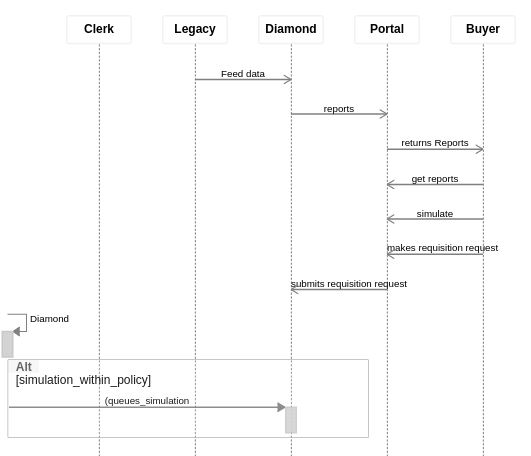
\includegraphics{Requisitions1.png}


\subsection{Intrinsic Information}
\label{Questions:intrinsic-information}

\subsection{Extrinsic Information}
\label{Questions:extrinsic-information}
Gather all information, it should all be available in the portal


\section{Related articles}
\label{Questions:related-articles}

\chapter{Service Level Agreements}
\label{Questions:service-level-agreements}

\chapter{Definitions}
\label{Questions:definitions}
Definitions:

\begin{Verbatim}[commandchars=\\\{\}]
ABC\_SLS\_PCT\_DLR

    Top 20 of previous 12 month contribution to sales dollars
    Does not adequately support new product introduction

ABC\_CUST\_QTE

SVC\_LVL

    Contractual service levels

ABC\_SLS\_PCT ABC Sales Percent
\end{Verbatim}


\chapter{ABC - Pareto}
\label{Portal/100-ABC::doc}\label{Portal/100-ABC:abc-pareto}

\section{Purpose}
\label{Portal/100-ABC:purpose}
Concentrate inventory and dollars on
\begin{itemize}
\item {} 
high volume,

\item {} 
high profit item

\item {} 
highest service level

\item {} 
core products

\item {} 
JIT / SLA / KITS

\end{itemize}

Metric


\section{Assumptions}
\label{Portal/100-ABC:assumptions}
Users wish to quickly summarize the characteristics of an item


\section{Item Statistics}
\label{Portal/100-ABC:item-statistics}

\section{Overview}
\label{Portal/100-ABC:overview}
This demonstrates computing a number of potentially useful statistics


\section{Definition}
\label{Portal/100-ABC:definition}
This is also known as Pareto or 80/20 rule

\href{https://en.wikipedia.org/wiki/Pareto\_principle}{https://en.wikipedia.org/wiki/Pareto\_principle}
\begin{itemize}
\item {} 
Top 20 percent of sales items are rated A

\item {} 
Next 60 percent rated B

\item {} 
Bottom 20 Rated C

\end{itemize}

This has the following problems, an item may be at 21\% but is indistinguishable from a 79


\section{Approach}
\label{Portal/100-ABC:approach}\begin{itemize}
\item {} 
Create a table to hold statistics

\item {} 
Create a script to populate statistics by item

\item {} 
Create a service to obtain the data model for the web page

\item {} 
create an angular 8 controller \emph{label-name}

\item {} 
Modify the filter screen to allow query filters on the statistics

\item {} 
Modify the web pages to show the statistics information

\end{itemize}


\section{Purpose}
\label{Portal/100-ABC:id1}
Concentrate inventory and dollars on
\begin{itemize}
\item {} 
high volume,

\item {} 
high profit item

\item {} 
highest service level for \textbf{important} products, those with high margins, not just hhigh

\end{itemize}

markups , complementery sales, Service Level Agreements, Just in Time Contracts and Kits.
\begin{itemize}
\item {} 
core products

\item {} 
{\color{red}\bfseries{}**}What should the service level be?  An item with a 5\% markup that turns 12 times a year may be

\end{itemize}

more profitable than an item with a 30\% markup and 1 annual turn**
\begin{quote}

\textbf{Certainly a B item at 21\% contriibution to profit margin is more valuable than a B item at 79\%.}
\end{quote}

package com.pacificdataservices.diamond.apsweb;

import java.io.IOException; import java.sql.Connection; import
java.sql.SQLException;

import javax.sql.DataSource;

import org.javautil.core.json.JsonSerializer; import
org.javautil.core.json.JsonSerializerGson; import
org.javautil.core.sql.Binds; import org.javautil.core.sql.SqlStatement;
import org.javautil.util.NameValue; import org.slf4j.Logger; import
org.slf4j.LoggerFactory; import
org.springframework.beans.factory.annotation.Autowired; import
org.springframework.web.bind.annotation.RequestMapping; import
org.springframework.web.bind.annotation.RequestParam; import
org.springframework.web.bind.annotation.RestController;

@RestController public class IcItemStatController \{
\begin{quote}

private Logger logger = LoggerFactory.getLogger(getClass());
@Autowired private DataSource datasource;
\end{quote}
\begin{description}
\item[{@RequestMapping(``/icItemStat'') public String planData(}] \leavevmode
@RequestParam(value=''itemNbr'') String itemNbr) throws SQLException,
IOException \{ \href{http://logger.info}{logger.info}(``invoked with
itemNumber \{\}'',itemNbr); Connection conn =
datasource.getConnection(); SqlStatement ss = new SqlStatement(conn,
``select * from ic\_item\_stat where item\_nbr = :item\_nbr''); Binds
binds = new Binds(); binds.put(``item\_nbr'', itemNbr); NameValue
nameValue = ss.getNameValue(binds,true); JsonSerializer serializer =
new JsonSerializerGson(); String json =
serializer.toJsonPretty(nameValue); return json; \}

\end{description}

{\color{red}\bfseries{}{}`}\href{https://www.briantracy.com/blog/personal-success/how-to-use-the-80-20-rule-pareto-principle/}{https://www.briantracy.com/blog/personal-success/how-to-use-the-80-20-rule-pareto-principle/} \textless{}\href{https://www.briantracy.com/blog/personal-success/how-to-use-the-80-20-rule-pareto-principle/}{https://www.briantracy.com/blog/personal-success/how-to-use-the-80-20-rule-pareto-principle/}\textgreater{}
\}


\subsection{Create a node service}
\label{Portal/100-ABC:create-a-node-service}

\section{Modify web page template}
\label{Portal/100-ABC:modify-web-page-template}
\href{https://en.wikipedia.org/wiki/Pareto\_principle}{https://en.wikipedia.org/wiki/Pareto\_principle}

\href{https://www.briantracy.com/blog/personal-success/how-to-use-the-80-20-rule-pareto-principle/}{https://www.briantracy.com/blog/personal-success/how-to-use-the-80-20-rule-pareto-principle/}


\section{Item Statistics}
\label{Portal/100-ABC:id6}

\section{Item Statistics Fields}
\label{Portal/100-ABC:item-statistics-fields}
\textbf{Name}

\textbf{Code}

\textbf{Description}

\textbf{Benefit}

\textbf{Disadvantage}

\textbf{Compare to}

While we are at it we may as well get
\begin{itemize}
\item {} 
Number of customers

\item {} 
Number of approved manufacturers

\item {} 
Annual Turns

\item {} 
Sales Conversion Percentile from quotes

\end{itemize}

ABC

ABC\_SLS

Top 20 of previous12 month contribution to sales dollars

Does not adequately support new product introduction

ABCUSTQUOTE

Top 20 percent of CUST OPEN Quotes

Similar to ABC


\section{Approach}
\label{Portal/100-ABC:id7}\begin{itemize}
\item {} 
Create a table to hold statistics

\item {} 
Create a script to populate statistics by item

\item {} 
Create a service to obtain the data model for the web pages

\item {} 
Modify the filter screen to allow query filters on the statistics

\item {} 
Modify the web pages to show the statistics information

\end{itemize}


\chapter{Optimal Replenishment Quantity}
\label{Portal/200-OptimalReplenishmentQuantity::doc}\label{Portal/200-OptimalReplenishmentQuantity:optimal-replenishment-quantity}

\section{Objectives}
\label{Portal/200-OptimalReplenishmentQuantity:objectives}\begin{itemize}
\item {} 
Highest Profit

\item {} 
Highest Customer Satisfaction

\item {} 
JITS / KITS / SLA

\end{itemize}


\chapter{Unit Cost}
\label{Portal/300-UnitCost::doc}\label{Portal/300-UnitCost:unit-cost}
During one of my calls with Peter he told me that he was reviewing
purchase orders a simple line such as ``Buyers don'`t buy the correct
quantities to get a good price'' was extended to:


\section{Compute Optimal Purchase Quantity}
\label{Portal/300-UnitCost:compute-optimal-purchase-quantity}

\section{Cost Types}
\label{Portal/300-UnitCost:cost-types}
Compute a projected per unit cost by solving the equation

unit\_cost = (setup\_cost / qty) + incremental cost

For two different known qty and prices (vendor quotes) using linear
algebra


\section{Graph this relationship}
\label{Portal/300-UnitCost:graph-this-relationship}
Find the ``price knee'' the first derivative of the function, the slope of
the tangent starts to level off (it asymptotically approaches 0, meaning
the limit is the unit cost doesn'`t decrease at all. Depending on setup
cost, incremental cost and annual consumption a three year supply may be
ten percent more than a one year supply, it may also be three times the
acquisition cost and additional carrying costs must be considered.

Vendor quotes should include this range of quantities, purchasing
quantities should be in this range, buys can be made and even scheduled
so that lower per unit costs can be realized.

During one of my calls with Peter he told me that he was reviewing
purchase orders a simple line such as ``Buyers don'`t buy the correct
quantities to get a good price'' was extended to:


\section{Compute Optimal Purchase Quantity}
\label{Portal/300-UnitCost:id1}
Compute a projected per unit cost by solving the equation

unit\_cost = (setup\_cost / qty) + incremental cost

For two different known qty and prices (vendor quotes) using linear
algebra


\section{Graph this relationsihip}
\label{Portal/300-UnitCost:graph-this-relationsihip}
Find the ``price knee'' the first derivative of the function, the slope of
the tangent starts to level off (it asymptotically approaches 0, meaning
the limit is the unit cost doesn'`t decrease at all. Depending on setup
cost, incremental cost and annual consumption a three year supply may be
ten percent more than a one year supply, it may also be three times the
acquisition cost and additional carrying costs must be considered.
by  vendor
Vendor quotes should include this range of quantities, purchasing
quantities should be in this range, buys can be made and even scheduled
so that lower per unit costs can be realized.
by  vendor


\chapter{Multiple Lead Times}
\label{Portal/400-MultipleLeadTimes:multiple-lead-times}\label{Portal/400-MultipleLeadTimes::doc}

\section{Overview}
\label{Portal/400-MultipleLeadTimes:overview}
Vendors may have drastically different lead times.


\section{Acquiring}
\label{Portal/400-MultipleLeadTimes:acquiring}
Data for lead times should be derived from the latest vendor quotes that is the longest lead tie from
the maximum effective date for a vendor quote.

Note that item\_nbr, the item surrogate key is not used, allowing you to
get vendor quotes for items that have not been set up;
\DUspan{keyword}{}\DUspan{keyword}{}\DUspan{name}{}\DUspan{keyword}{}\DUspan{keyword}{}\DUspan{name}{}\DUspan{punctuation}{}\DUspan{name}{}\DUspan{punctuation}{}\DUspan{name}{}\DUspan{punctuation}{}\DUspan{keyword}{}\DUspan{punctuation}{}\DUspan{name}{}\DUspan{punctuation}{}\DUspan{name}{}\DUspan{punctuation}{}\DUspan{punctuation}{}\DUspan{keyword}{}\DUspan{punctuation}{}\DUspan{name}{}\DUspan{punctuation}{}\DUspan{operator}{}\DUspan{name}{}\DUspan{punctuation}{}\DUspan{operator}{}\DUspan{literal,number,integer}{}\DUspan{name}{}\DUspan{keyword}{}\DUspan{name}{}\DUspan{keyword}{}\DUspan{keyword}{}\DUspan{name}{}\DUspan{punctuation}{}\DUspan{name}{}\DUspan{punctuation}{}\DUspan{name}{}\DUspan{punctuation}{}\DUspan{name}{}\DUspan{punctuation}{}
\begin{Verbatim}[commandchars=\\\{\}]
create view ic\_item\_vnd\_lead\_time as
select  item\_cd\_qte,
    vq\_qte\_dt,
    vq\_qte\_eff\_dt,
    max(vq\_qte\_exp\_dt) max\_qte\_exp\_dt,
    (max(vq\_qte\_exp\_dt) - vq\_qte\_eff\_dt) / 7 lead\_tm\_wks
from vq\_qte\_vw
group by org\_nbr\_vnd,
    item\_cd\_qte,
    vq\_qte\_eff\_dt,
    vq\_qte\_dt;
\end{Verbatim}


\section{YAML}
\label{Portal/400-MultipleLeadTimes:yaml}
\begin{Verbatim}[commandchars=\\\{\}]
ic\_item\_vnd\_lead\_tm:
    sql: \textgreater{}
          create view ic\_item\_vnd\_lead\_time as
          select item\_cd\_qte,
               vq\_qte\_dt,
               vq\_qte\_eff\_dt,
               max(vq\_qte\_exp\_dt) max\_qte\_exp\_dt,
               (max(vq\_qte\_exp\_dt) - vq\_qte\_eff\_dt) / 7 lead\_tm\_wks
           from vq\_qte\_vw
           group by org\_nbr\_vnd,
              item\_cd\_qte,
              vq\_qte\_eff\_dt,
              vq\_qte\_dt;
     description: Create ic\_item\_vnd\_lead\_tm
     narrative: \textgreater{}
        TODO describe consequence of using the quote expiration date, vq\_qte\_exp\_dt
        rather than the quote of quotation or the effective date of quotation.
\end{Verbatim}


\section{Assumptions}
\label{Portal/400-MultipleLeadTimes:assumptions}
The most recent vendor quote for lead times will be used.

If multiple vendor quotes exist for the same quote date, the maximum
lead time will be used.

Full historical vendor quotes are useful to see trends in cost and lead
time.


\section{Issues}
\label{Portal/400-MultipleLeadTimes:issues}
Vendor on-time performance.


\chapter{Lead Time By Vendor}
\label{Portal/450-MultipleLeadTimes2:lead-time-by-vendor}\label{Portal/450-MultipleLeadTimes2::doc}

\section{Overview}
\label{Portal/450-MultipleLeadTimes2:overview}
Vendors may have drastically different lead times.


\section{Acquiring}
\label{Portal/450-MultipleLeadTimes2:acquiring}
Data for lead times should be derived from the latest vendor quotes that is:

Note that item\_nbr, the item surrogate key is not used, allowing you to
get vendor quotes for items that have not been set up;
\DUspan{keyword}{}\DUspan{keyword}{}\DUspan{name}{}\DUspan{keyword}{}\DUspan{keyword}{}\DUspan{name}{}\DUspan{punctuation}{}\DUspan{name}{}\DUspan{punctuation}{}\DUspan{name}{}\DUspan{punctuation}{}\DUspan{keyword}{}\DUspan{punctuation}{}\DUspan{name}{}\DUspan{punctuation}{}\DUspan{name}{}\DUspan{punctuation}{}\DUspan{punctuation}{}\DUspan{keyword}{}\DUspan{punctuation}{}\DUspan{name}{}\DUspan{punctuation}{}\DUspan{operator}{}\DUspan{name}{}\DUspan{punctuation}{}\DUspan{operator}{}\DUspan{literal,number,integer}{}\DUspan{name}{}\DUspan{keyword}{}\DUspan{name}{}\DUspan{keyword}{}\DUspan{keyword}{}\DUspan{name}{}\DUspan{punctuation}{}\DUspan{name}{}\DUspan{punctuation}{}\DUspan{name}{}\DUspan{punctuation}{}\DUspan{name}{}\DUspan{punctuation}{}
\begin{Verbatim}[commandchars=\\\{\}]
create view ic\_item\_vnd\_lead\_time as
select  item\_cd\_qte,
    vq\_qte\_dt,
    vq\_qte\_eff\_dt,
    max(vq\_qte\_exp\_dt) max\_qte\_exp\_dt,
    (max(vq\_qte\_exp\_dt) - vq\_qte\_eff\_dt) / 7 lead\_tm\_wks
from vq\_qte\_vw
group by org\_nbr\_vnd,
    item\_cd\_qte,
    vq\_qte\_eff\_dt,
    vq\_qte\_dt;
\end{Verbatim}


\section{YAML}
\label{Portal/450-MultipleLeadTimes2:yaml}\begin{description}
\item[{ic\_item\_vnd\_lead\_tm:}] \leavevmode\begin{description}
\item[{sql: \textgreater{}}] \leavevmode\begin{quote}

create view ic\_item\_vnd\_lead\_time as
select item\_cd\_qte,
\begin{quote}
\begin{quote}

vq\_qte\_dt,
vq\_qte\_eff\_dt,
max(vq\_qte\_exp\_dt) max\_qte\_exp\_dt,
(max(vq\_qte\_exp\_dt) - vq\_qte\_eff\_dt) / 7 lead\_tm\_wks
\end{quote}

from vq\_qte\_vw
group by org\_nbr\_vnd,
\begin{quote}

item\_cd\_qte,
vq\_qte\_eff\_dt,
vq\_qte\_dt;
\end{quote}
\end{quote}
\end{quote}

description: Create ic\_item\_vnd\_lead\_tm
narrative: \textgreater{}
\begin{quote}

TODO describe consequence of using the quote expiration date, vq\_qte\_exp\_dt
rather than the quote of quotation or the effectivedate of quotation.
\end{quote}

\end{description}

\end{description}


\section{Assumptions}
\label{Portal/450-MultipleLeadTimes2:assumptions}
The most recent vendor quote for lead times will be used.

If multiple vendor quotes exist for the same quote date, the maximum
lead time will be used.

Full historical vendor quotes are useful to see trends in cost and lead
time.


\section{Issues}
\label{Portal/450-MultipleLeadTimes2:issues}
Vendor on-time performance.

TODO flesh out


\chapter{Business Process Improvement : Create Requisition}
\label{Portal/700-Create-Requisition:business-process-improvement-create-requisition}\label{Portal/700-Create-Requisition::doc}\begin{enumerate}
\item {} 
Business Process Improvement

\item {} 
Project Description

\item {} 
Diamond Portal

\item {} 
Portal Functionality

\item {} 
Purchasing

\end{enumerate}


\section{Business Process Improvement : Create Requisition}
\label{Portal/700-Create-Requisition:id1}
Created by James Schmidt, last modified on Dec 21, 2019

{]}How and why to create a requisition


\subsection{Instructions}
\label{Portal/700-Create-Requisition:instructions}\begin{enumerate}
\item {} 
Look at the report section of the portal

\item {} 
Review the information

\item {} 
Fill out the checkist

\item {} 
Create the requistitio

\end{enumerate}


\subsubsection{Requisition Checklist}
\label{Portal/700-Create-Requisition:requisition-checklist}

\subsection{Sequence Diagram}
\label{Portal/700-Create-Requisition:sequence-diagram}
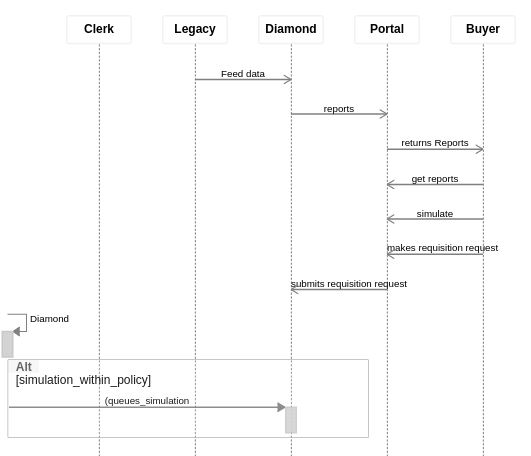
\includegraphics{Requisitions.png}


\subsubsection{Intrinsic Information}
\label{Portal/700-Create-Requisition:intrinsic-information}

\subsubsection{Extrinsic Information}
\label{Portal/700-Create-Requisition:extrinsic-information}
Gather all information, it should all be available in the portal


\subsection{Related articles}
\label{Portal/700-Create-Requisition:related-articles}

\chapter{Requisition}
\label{Portal/750-Requisitions:requisition}\label{Portal/750-Requisitions::doc}
{]}How and why to create a requisition


\section{Instructions}
\label{Portal/750-Requisitions:instructions}\begin{enumerate}
\item {} 
Look at the report section of the portal

\item {} 
Review the information

\item {} 
Fill out the checkist

\item {} 
Simulate

\item {} 
Create the requisititioni

\item {} 
Proper quantity for ABC?

\end{enumerate}


\section{Gather Information}
\label{Portal/750-Requisitions:gather-information}\begin{itemize}
\item {} 
Lead Times

\item {} 
Unit Costs

\item {} 
Optimal Replenishment Quantities

\item {} 
Approved Manufacturers

\end{itemize}


\subsection{Requisition Checklist}
\label{Portal/750-Requisitions:requisition-checklist}

\subsection{Intrinsic Information}
\label{Portal/750-Requisitions:intrinsic-information}

\subsection{Extrinsic Information}
\label{Portal/750-Requisitions:extrinsic-information}

\subsection{Simulate}
\label{Portal/750-Requisitions:simulate}
DOCTHIS


\subsection{Sequence Diagram}
\label{Portal/750-Requisitions:sequence-diagram}
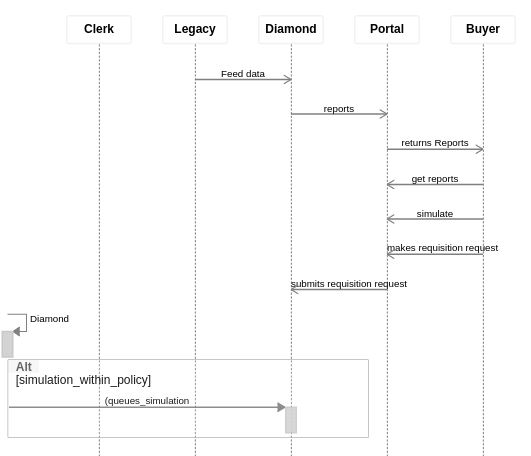
\includegraphics{Requisitions.png}
\begin{enumerate}
\item {} 
What are the requisition review requirements?
\begin{itemize}
\item {} 
When is a requisition subject to review?

\item {} 
What are the needs additional work conditions?
\begin{itemize}
\item {} 
Need more vendor quotes

\item {} 
Need work on equivalent parts

\item {} 
Incorrect buy quantity

\item {} 
Get existing inventory certified.

\end{itemize}

\end{itemize}

\end{enumerate}


\section{Out of Scope}
\label{Portal/750-Requisitions:out-of-scope}
Lead times can vary drastically based on
\begin{itemize}
\item {} 
vendor

\item {} 
material shortages

\item {} 
new product introduction

\item {} 
product recall MRO (Maintenance, Repair and Overhaul)Definition

\end{itemize}

The elapsed time, usually measured in weeks between when a product
is ordered and receivied.

Usually not considered
\begin{itemize}
\item {} 
Recieving time

\item {} 
Inspection Time

\item {} 
Intra-facility transfer time

\item {} 
These are consider \emph{availability times}

\end{itemize}

Typically in DRP Planning
\begin{itemize}
\item {} 
There is only one lead time

\item {} 
This lead time is fairly consistent

\item {} 
Costs due not vary based on lead time.

\end{itemize}


\section{In aerospace}
\label{Portal/750-Requisitions:in-aerospace}

\section{Source of Lead Time}
\label{Portal/750-Requisitions:source-of-lead-time}

\subsection{vendor quotes}
\label{Portal/750-Requisitions:vendor-quotes}
Take the lead time from the maximum quote expiration date


\subsection{Summarized Lead Times should include}
\label{Portal/750-Requisitions:summarized-lead-times-should-include}\begin{itemize}
\item {} 
Vendor Code

\item {} 
Vendor type (Manufacturer, Distibutor, intra-company

\item {} 
Vendor quote beginning and ending effective date

\item {} 
Date of request for quote

\end{itemize}


\subsection{Lead time details should include:}
\label{Portal/750-Requisitions:lead-time-details-should-include}\begin{itemize}
\item {} 
Historical lead times

\end{itemize}


\subsection{Lead time projections}
\label{Portal/750-Requisitions:lead-time-projections}
Factors that can effect lead time, Lead times can vary drastically based
on
\begin{itemize}
\item {} 
vendor

\item {} 
Some vendors will stock

\item {} 
Some manufacturers will build to stock

\item {} 
Some manufactureres will build only on demand, see Cost per Unit

\item {} 
material shortages

\item {} 
new product introduction

\item {} 
product recall MRO (Maintenance, Repair and Overhaul)

\end{itemize}

\begin{DUlineblock}{0em}
\item[] 
\end{DUlineblock}


\section{Instructions}
\label{Portal/750-Requisitions:id1}\begin{enumerate}
\item {} 
Look at the report section of the portal

\item {} 
Review the information

\item {} 
Fill out the checklist

\item {} 
Create the requisition

\end{enumerate}


\subsection{Requisition Checklist}
\label{Portal/750-Requisitions:id2}

\section{Sequence Diagram}
\label{Portal/750-Requisitions:id3}
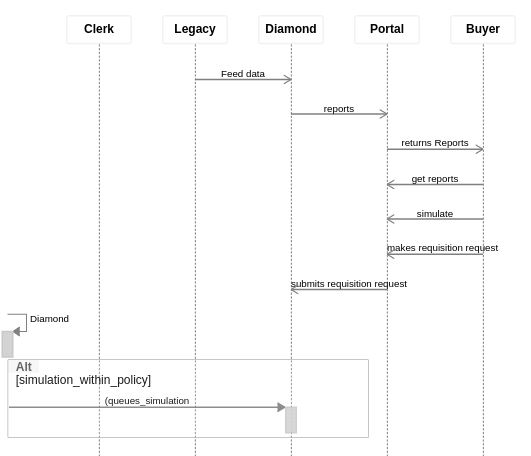
\includegraphics{Requisitions.png}


\subsection{Intrinsic Information}
\label{Portal/750-Requisitions:id4}

\subsection{Extrinsic Information}
\label{Portal/750-Requisitions:id5}
Gather all information, it should all be available in the portal


\section{Related articles}
\label{Portal/750-Requisitions:related-articles}

\chapter{Airframe Scenario 737 Max}
\label{Portal/800-737max:airframe-scenario-737-max}\label{Portal/800-737max::doc}
As Boeing grounds planes and stops manufacturing 737 Max,

lead times from and costs from distributors are presumably dropping, but client would carry until ramp up resumes. Can they be bought at manufacturer costs now and sat on until production resumes?  Lower acquisition cost, higher carrying costs and intermediate turns will be non existent but risk of obsolescence decreases. We can only plug in the variables and run various simulations or a Monte Carlo simulation.

All intrinsic system information for my formulas is worthless in this scenario.

Buy a bunch of parts at lower cost now and take delivery now from distributors or buy for delivery in 30 weeks?  When will production resume?   These are judgment calls based communication with the manufacturer.  The distributors are probably offering for less, the lead times should be shorter, the costs less, but the will sit idle for six to eighteen months.

We can only plug in these assumptions and come up with buys based on those assumptions, historical data in the system has significantly less value.  We can only come up with investment cost and carrying cost based on this extrinsic information and the formulas I have developed but not yet published.

..image:: Portal/images/ActionReport.png


\chapter{Indices and tables}
\label{index:indices-and-tables}\begin{itemize}
\item {} 
\emph{genindex}

\item {} 
\emph{modindex}

\item {} 
\emph{search}

\end{itemize}



\renewcommand{\indexname}{Index}
\printindex
\end{document}
